\chapter{System zur Visualisierung von Schmerz Scores am Beispiel akustischer Signale}

Das in dieser Arbeit umzusetzende System muss den folgenden Anforderungen genügen:
\begin{enumerate}
	\item Das System muss dazu in der Lage sein, aus den akustischen Eigenschaften des Weinens eines Babys den Schmerz Score bezüglich einer Pain Scale abzuleiten.
	\item Das System muss dazu in der Lage sein, die abgeleiteten Schmerz Scores zu visualiseren.
	\item Das System muss dazu in der Lage sein, beliebige Pain Scales einzubinden. 
	\item Die System muss dazu in der Lage sein,  die Analyse auch bei nicht-optimalen akustischen Bedingungen durchzuführen.
	\item Das System muss dazu in der Lage sein, die Analyse kontinuierlich durchzuführen.
\end{enumerate}

\section{Literaturüberblick}
\label{sec:system_literature}

In diesem Kapitel wird ein Überblick über bereits veröffentlichte Ansätze zur Analyse akustischer Signale von Neugeborenen gegeben.

Ein großer Teil der Veröffentlichungen stellt Algorithmen zur Klassifizierung einzelner Cry Units vor, entweder bezüglich der Weinursache (Hunger, Angst, Schmerz, ... ) oder zur Diagnose bestimmter Krankheiten. Diese Methoden sind in den meisten Fällen nicht für die kontinuierliche Analyse geeignet, sondern haben das Ziel, eine gegebenen Cry-Unit mit einer möglichst hohen Genauigkeit bezüglich der Ursache zu klassifizieren. Probleme wie Hintergrundrauschen, Berechnungsaufwand oder kontextuelle Informationen spielen eine untergeordnete Rolle. Beispiele für solche Veröffentlichungen sind die von Abdulaziz et al. \cite{class_abdulaziz} oder Fuhr et al. \cite{comparisonOfLearning}.

Várallyay stellte in seiner Dissertation \glqq Analysis of the Infant Cry with Objective Methods\grqq{} \cite{cry_thesis} Methoden zur automatisierten Analyse kindlicher Lautäußerungen vor. Das primäre Ziel der Dissertation war die Erforschung der Unterschiede zwischen den Lautäußerungen gesunder und tauber Neugeborener. Die Algorithmen zur automatisierten Analyse der Audiosignale waren ein \glqq Nebenprodukt\grqq{} zur schnelleren Datenauswertung. Die Auswertung musste nicht kontinuierlich erfolgen. In der vorgestellten Verarbeitungspipeline wurde das Eingangssignal in Zeitfenster weniger Millisekunden zerlegt und jedes Fenster nach Entscheidungsregeln als \emph{stimmhaft} oder \emph{nicht stimmhaft} markiert. Die stimmhaften Signalfenster wurden zu \emph{Segmenten} zusammengefasst (welche in Kapitel \ref{sec:acousticModel} als Cry-Units bezeichnet werden). Auf Basis der Segmente wurden Auswertungen bezüglich des Zeitbereiches (Durchschnittliche Segmentlänge, Pausenlängen etc.), des Frequenzbereiches (Grund-Frequenz, Formanten-Frequenzen etc.) und des Melodieverlaufes angestellt. Analysiert wurden Audioaufnahmen von Babys mit einer Länge von 10 bis \SI{100}{\second}. Aus den Auswertungsergebnisse stellte Varallyay die wichtigsten Unterscheidungsmerkmale zwischen tauben und gesunden Babys fest. In der Dissertation \cite{cry_thesis} wird ein Überblick über das Vorgehen und die Ergebnisse gegeben. Die Verarbeitungsschritte wurden detaillierter in einzelnen Veröffentlichungen beschrieben, wobei der Autor dieser Arbeit nur den Zugriff auf einige dieser Veröffentlichungen erhalten konnte.

Cohen et al. haben 2012 in der Veröffentlichung \glqq Infant Cry Analysis and Detection\grqq{} \cite{cohenCry}  ein System zur Analyse der akustischen Signale von Neugeborenen vorgestellt. Dieses System klassifizierte die Audiosignale in eine der drei Klassen \emph{Cry, No Cry} und \emph{No Activity}. Die Klasse \emph{Cry} bezeichnet Lautäußerungen, die eine potentiell Gefahr für das Baby anzeigen, wie z.B. wie Schmerz oder Hunger. Die Klasse \emph{No Cry} bedeutete, dass das Baby zwar Laute von sich gibt, diese aber keine potentielle Gefahr anzeigen. Die Klasse \emph{No Activity} bezeichnete keinerlei Lautäußerung. Die Verarbeitungs-Pipeline wurde detailliert vorgestellt und war für die kontinuierliche Verarbeitung mit einer gewissen Verzögerungszeit spezialisiert. Das Signal wird in überlappende \emph{Segmente} \`{a} \SI{10}{\second} zerlegt. Die Stimmaktivität in den Segmenten wird algorithmisch festgestellt. Wenn Aktivität vorliegt, wird das Segment in Sektionen \`{a} \SI{1}{\second} zerlegt und die Stimmaktivität für jede Sektion gemessen. Wird genügend Stimmaktivität in einer Sektion festgestellt, wird die Sektion in \emph{Frames} \`{a} \SI{32}{\milli\second} zerlegt und Attribute für jeden Frame errechnet. Mit Hilfe von Entscheidungsregeln werden die Frames in \emph{Cry, No-Cry} oder \emph{No Activity} klassifiziert, wobei kontextuelle Informationen der umliegenden Frames mit einbezogen werden. Aus den Klassen der Frames wird auf die Klasse der Sektion geschlossen, und aus den Klassen der Sektionen auf die Klasse des Segmentes. Das System hat mit den Anforderungen dieser Arbeit gemeinsam, dass ebenfalls die kontinuierliche Verarbeitung im Vordergrund steht. Der Nachteil an dieser Methode ist, dass die zeitliche längste Einheit, für die die Klassifizierung vorgenommen wird, unflexibel auf \SI{10}{\second} festgelegt ist. Daher müsste diese Verarbeitungs-Pipeline abgewandelt werden, um anstelle der Ableitung der drei genannten Klassen einen Pain Score ableiten zu können, die einen längeren Beobachtungszeitraum als \SI{10}{\second} benötigt.

Pal et al.  haben 2006 in der Veröffentlichung \glqq Emotion detection from infant facial experessions and cries\grqq{} \cite{palEmotion} ein System vorgestellt, welches aus den akustischen Eigenschaften des Weinens die Emotion ableitet. Die zu erkennenden Emotionen sind \emph{Traurigkeit, Wut, Hunger, Angst und Schmerz}. Es wird nicht erwähnt, ob die Analyse kontinuierlich oder nicht kontinuierlich erfolgt. Bei der Verarbeitung der akustischen Signale werden die Attribute \emph{Grundtonhöhe} und die \emph{Frequenz der ersten drei Formanten} extrahiert und mit einem Klassifizierungsalgorithmus klassifiziert. Es wurde nicht beschrieben, inwiefern die Eigenschaften aus kurzen Signalfenstern oder längeren Signalabschnitten errechnet werden, welche Vorverarbeitungsschritte angewandt werden und ob die Klassifizierung auf Ebene der Signalfenster oder über längere Zeitabschnitte hinweg geschieht.

Zamzi et al.  haben 2016 in der Veröffentlichung \glqq An Approach for Automated Multimodal Analysis of Infants' Pain\grqq{} \cite{zamziMultimodal} ein System zur automatisierten und kontinuierlichen multimodalen Analyse von Neugeborenen zur Ableitung des Schmerzes vorgestellt. Das System trägt den Namen \emph{MPAS}. Der Schmerzgrad wird aus den Analyseergebnissen der monomodalen Schmerzindikatoren für \emph{Gesichtsausdruck, Körperbewegung, Vitalfunktionen und Weinen} errechnet. Das System kommt der Aufgabenstellung dieser Masterarbeit am nächsten, da es ebenfalls um die Ableitung von Schmerz in einem multimodalen Verbund geht. Der Schmerz wurde hier \glqq direkt\grqq{} abgeleitet, ohne den Weg über Pain Scales zu wählen. Während in der Veröffentlichung die Analyse der ersten drei genannten Schmerzindikatoren angekündigt wurde, wurden daraufhin die Methoden zur Analyse der akustischen Signale \emph{nicht} erläutert. Auch die ersten Validierungsergebnisse beziehen sich nur auf den Gesichtsausdruck, die Körperbewegung und die Vitalfunktionen. Es ist nicht klar, ob die Miteinbeziehung akustischer Signale fallen gelassen wurde. Die Ausführungen konzentrieren sich dazu vermehrt auf die Methoden zur Kombination der Auswertungsergebnisse der monomodalen Schmerzindikatoren.

\section{Verarbeitungs-Pipeline}

In Kapitel \ref{sec:system_literature} wurden verschiedene Systeme vorgestellt, deren Zielstellungen dem Thema dieser Masterarbeit ähneln. Keine der präsentierten Verarbeitungs-Pipelines eignet sich, um mit nur leichten Anpassungen übernommen werden zu können: Entweder wurden die Verarbeitungsschritte nicht für die kontinuierliche Verarbeitung konzipiert \cite{class_abdulaziz} \cite{comparisonOfLearning} \cite{cry_thesis}, nicht genügen abstrahiert, um für andere Klassifizierungen als die ursprünglich geplanten abgewandelt werden zu können \cite{cohenCry}, oder die Verarbeitungs-Pipeline wurde nicht vorgestellt. \cite{palEmotion} \cite{zamziMultimodal}.

In dieser Arbeit wird die folgende Verarbeitungs-Pipeline entworfen. Sie wird in in Abbildung \ref{img:architecture-overview} visualisiert. 

\begin{enumerate}[leftmargin=*]
	\item \textbf{Vorverrbeitung} (engl. \emph{Pre-Processing}) des Signals, beschrieben in Kapitel \ref{sec:preprocessing}.
	
	\item \textbf{Voice Activity Detection}. Das Audiosignal wird in einander überlappende Zeitfenster weniger Millisekunden  aufgeteilt. Mit Hilfe eines Klassifizierungsalgorithmus werden die Zeitfenster in als \emph{stimmhaft} oder \emph{nicht stimmhaft} markiert. Ununterbrochene Reihen stimmhafter Signalfenstern werden zu \emph{Cry-Units} zusammengefasst, welche die Grundlage der darauf folgenden Verarbeitungsschritte bilden. Diese Idee wurde aus der Dissertation von Várallyay \cite[S. 16 - 17]{cry_thesis} übernommen, welcher Cry-Units als \emph{Segmente} bezeichnet. Die Voice Activity Detection wird in Kapitel \ref{sec:vad} vorgestellt.
	
	\item \textbf{Segmentierung} (engl \emph{Segmenting}). Die Cry-Units werden zu Segmenten zusammengefasst. Dieser Schritt ist notwendig, weil die Ableitung des Schmerz Score nicht aus den Informationen einer Cry-Unit, sondern aus dem Verbund mehrerer Cry-Units geschieht. Keine der in Kapitel \ref{sec:system_literature} vorgestellten Veröffentlichungen beschreibt ein Verfahren, welches adaptiert werden könnte. Daher wird ein simpler Algorithmus für die Segmentierung vorgeschlagen, welcher für eine kontinuierliche Auswertung implementiert werden kann. Die Segmentierung wird in Kapitel \ref{sec:segmenting} vorgestellt.		
	
	\item \textbf{Extrahierung von Eigenschaften} (engl. \emph{Feature Extraction}), das heißt die Berechnung von Features für jedes Segment, aus denen der Schmerz Score abgeleitet werden kann. Dieser Prozess wird in Kapitel \ref{sec:segmentFeatures} vorgestellt.	
	
	\item \textbf{Ableitung der Schmerz Score} (engl. \emph{Prediction of Pain Score}) aus den Eigenschaften der Segmente. Dieses Problem kann entweder als Klassifizierungs- oder Regressionsaufgabe modelliert werden. Die grundlegende Idee wird in Kapitel \ref{sec:overviewPainRegression} vorgestellt und in Kapitel \ref{sec:regressionPainScore} weiter ausgearbeitet.
	
	\item \textbf{Visualisierung} (engl. \emph{Visualisation}) der abgeleiteten Schmerz Score. In dieser Arbeit werden mehrere Varianten vorgeschlagen, welche die Höhe des Schmerz Score in seinem zeitlichen Verlauf auf Ampelfarben abbildet. Die Visualisierung wird in Kapitel \ref{sec:visualisation}	vorgestellt.
\end{enumerate}

\begin{figure}[H]
	\centering
	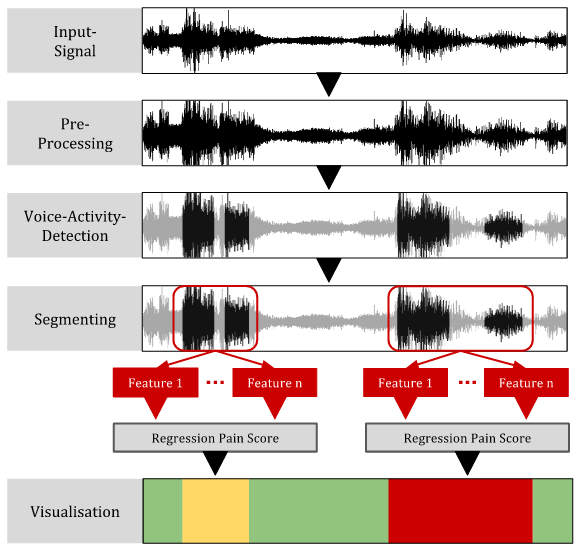
\includegraphics[width=0.75\textwidth]{bilder/pipeline01.png}
	\caption{Überblick über die Verarbeitungs-Pipeline dieser Arbeit}
	\label{img:architecture-overview}
\end{figure}

\section{Vorverarbeitung}
\label{sec:preprocessing}

Bei der Vorverarbeitung wird das Signal so manipuliert, dass Störeinflüsse auf die darauf folgenden Verarbeitungsschritte minimiert werden. Welche Vorverarbeitung durchgeführt wird, ist Abhängig von der konkreten Aufgabenstellung. So werden beispielsweise bei einigen Algorithmen zur Voice Activity Detection, also dem markieren stimmhafter Signalabschnitte, Tiefpass, Hochpass- und Bandpassfilter eingesetzt, um diejenigen Frequenzanteile herauszufiltern, die von der Stimme nicht produziert werden können \cite{vad_entropy} \cite{vad_ceps} \cite{vad_kola}. Bei einigen Tonhöhenerkennungsalgorithmen wird \emph{Centerclipping} eingesetzt, also das 0-Setzen von Samples mit $ x[i] < 0.5 \cdot \maxi\{x[\;]\}$.\cite{czechPitch} 

In dieser Arbeit wurde sich für eine Vorverarbeitung entschieden, bei der das Signal hinsichtlich seiner Dynamik im Zeitbereich eingeschränkt wird. Dies ist ein typischer Vorverarbeitungschritt bei Sprachaufnahmen. Hintergrund ist, dass sehr kurze Pegelspitzen, deren Pegel weit über dem Durchschnittspegel liegen, die durchschnittliche Energie des Signals unnötig niedrig halten. Da die Testsignale, die in dieser Arbeit verwendet wurden, aus inhomogenen Quellen stammen und sehr unterschiedliche Lautstärken haben, sollte so eine annähernde Angleichung der Signalenergien erreicht werden. An dieser Stelle werden noch keine Frequenzanteile herausgefiltert, da ansonsten Frequenzen verloren werden können, die in den späteren Verarbeitungsschritten eventuell noch benötigt werden.

Die Dynamikeinschränkung wird mit Hilfe eines Audio-Kompressors umgesetzt. Dieser verringert Signalspitzen, die über einen festgelegten \emph{Schwellwert} (engl. \emph{Threshold}) $\theta$ liegen, um ein festgelegtes \emph{Verhältnis} (engl. \emph{Ratio)} $\rho$. Ein Schwellwert von $\theta = 0.3$ mit einem Verhältnis von $\rho = 0.5$ bedeutet beispielsweise, dass alle Signalspitzen, die den Wert 0.3 über-, oder $-0.3$ unterschreiten, um 50\% verringert werden. Der Wert eines Samples nach der Kompression $x_{comp}[n]$ ergibt sich somit nach Gleichung \ref{eq:preprocessedX}.

\begin{equation}
\text{comp}(x[n], \theta, \rho) =
\begin{cases}
\theta + (x[n] - \theta) \rho \quad , \text{wenn } x[n] > \theta \\
-\theta + (x[n] + \theta) \rho \quad, \text{wenn } x[n] < -\theta \\
x[n] \quad \text{sonst}
\end{cases}
\label{eq:preprocessedX}
\end{equation}

Die Amplituden hoherer Signalspitzen werden so verringert, wodurch Headroom gewonnen wird, welcher anschließend bei der gleichmäßigen Erhöhung aller Amplituden zur Erhöhung der insgesamten Energie genutzt werden kann. Diese Erhöhung kann beispielsweise durch eine Normalisierung nach Gleichung \ref{eq:normalizing} durchgeführt werden.

\begin{equation}
\text{normalize}(x[n]) = \frac{x[n]}{\maxi\{x[\;]\}}
\label{eq:normalizing}
\end{equation}

Bei dem Kompressor, der in dieser Verarbeitungs-Pipeline zur Vorverarbeitung verwendet wird, werden Threshold und Ratio nach Formel \ref{eq:THold} als Funktion des RMS-Wertes des Signals berechnet. Der Parameter $r_a$ gibt den Ziel-RMS-Wert an. Der RMS-Wert wird nach Formel \ref{eq:rms} berechnet.

\begin{equation}
\theta(x[\;]) = \rho(x[\;])  = \bigg[\frac{\text{RMS}(x[\;])}{r_a}\bigg]^{2}
\label{eq:THold}
\end{equation}

Die Vorverarbeitung wird durchgeführt, indem (1.) die Kompression mit den Parametern nach Gleichung \ref{eq:THold} und (2.) die Normalisierung nach Gleichung \ref{eq:THold} durchgeführt wird. Abbildung \ref{img:compressing01} zeigt ein Signal vor und nach der Vorverarbeitung nach diesem Prinzip.

\begin{figure}[h]
	\centering
	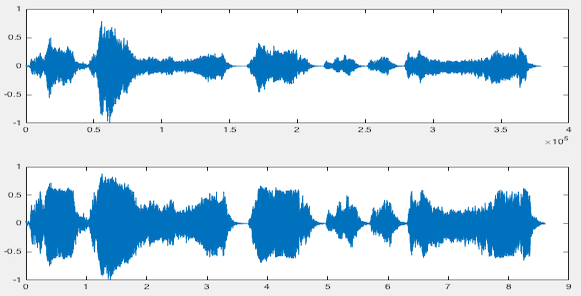
\includegraphics[width=0.7\textwidth]{bilder/compressing01.png}
	\caption{Ergebnis der Vorverarbeitung. Oben: Das Signal vor der Vorverarbeitung. Unten: Das Signal nach der Vorverarbeitung.}
	\label{img:compressing01}
\end{figure}

Damit diese Vorverarbeitung kontinuierlich eingesetzt werden kann, wird vorgeschlagen, den Kompressor mit \grqq sanften Werten\grqq{} zu initialisieren, wie zum Beispiel $\theta = \rho = 0.7$ und $\maxi\{x[\;] = 0.9\}$. Diese Parameter können nach der Beendigung eines Segmente auf Basis des RMS-Wertes des Segmentes aktualsisiert und für die Vorverarbeitung der zukünftigen Werte eingesetzt werden (Siehe Kapitel \ref{sec:segmenting}). Um eine zu große Beeinflussung des Signals zu vermeiden, wurde ein Minimalwert für Threshold und Ratio von $0.4$ festgelegt.

\section{Voice Activity Detection}
\label{sec:vad}

Das Ziel ist, in einem Audiosignal diejenigen Stellen zu markieren, in denen Stimme enthalten ist. Abbilung \ref{img:vad01} visualisiert ein Beispiel für eine solche Markierung. Zu sehen ist der Zeitbereich eines Audiosignales mit fünf klar erkennbaren Cry-Units. Die rote Linie, die das Signal überspannt, bildet die Zeiteinheiten des Eingangssignales in die binären Kategorien $1 hat{=} $ \emph{stimmhaft} (engl. \emph{voiced}) und $0 hat{=}  $ \emph{Stille} (oder \emph{nicht-stimmhaft}, engl. \emph{not voiced}) ab.

\begin{figure}[h]
	\centering
	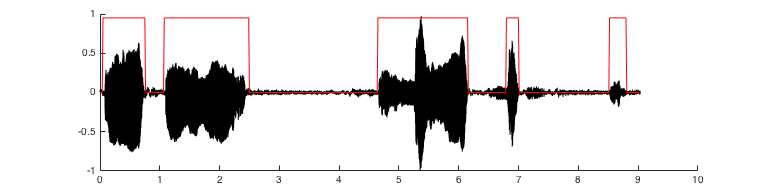
\includegraphics[width=0.7\textwidth]{bilder/vad_introduction01.png}
	\caption{Markierung stimmhafter Bereiche in einem Audiosignal. Schwarz: Das Eingangssignal $x[\;]$. Rot: Klassifizierung in stimmhaft/Stille. Es sind fünf Cry-Units zu erkennen.}
	\label{img:vad01}
\end{figure}

Die Erkennung des Vorhandenseins von Stimme in einem Signal wird als \emph{Voice Activity Detection (VAD)} oder auch \emph{Speech Detection} bezeichnet. Das Ziel ist die Unterscheidung von denjenigen Zeiträumen im Signal, in denen Stimme enthalten ist, von den Zeiträumen ohne Stimme. Die größte Herausforderung für VAD-Algorithmen ist die robuste Erkennung bei Signalen mit Rauschen unbekannter Stärke und Natur. \cite[S. 1]{vad_kola} \cite[S. 1]{vad_Lisboa}

Der Grundlegende Aufbau eines VAD-Algorithmus ist wie folgt.
\begin{enumerate}
\item \textbf{Windowing:} Unterteilung des Signals in (einander überlappende) Signalfenster.
\item \textbf{Extraktion von Eigenschaften} aus den einzelnen Signalfenstern.
\item \textbf{Entscheidung} über die Präsens oder Abwesenheit von Stimme für jedes Signalfenster auf Grundlage der extrahierten Attribute mit Hilfe von Entscheidungsregeln wie Grenzwerten.
\item \textbf{Decision-Smoothing}, das nachträgliche Hinzufügen oder Entfernen von Entscheidungen mit Hilfe von kontextuellen Informationen der umliegenden Entschiedungen.\cite[S. 8 - 9]{vad_granada} \cite[S. 1 - 2]{vad_kola}
\end{enumerate}

Auch die in dieser Arbeit durchgeführte Voice Activity Detection folgt diesem Schema. Das Windowing wird in Kapitel \ref{sec:windowing}, die Extraktion von Eigenschaften in Kapitel \ref{sec:featExtraction}, die Entscheidung in Kapitel \ref{sec:vad_thresholding} und das Decision-Smoothing in Kapitel \ref{sec:smoothing} beschrieben. Es wurden Ideen verwendet, die von  Moattar et al. \cite{vad_Easy}, Kristjansson et al. \cite{vad_Lisboa}, Waheed et al. \cite{vad_entropy}, Ahmadi et al. \cite{vad_ceps} und Shen et al.\cite{vad_entropie02} vorgestellt wurden.

\subsection{Windowing}
\label{sec:windowing}

Wird die Voice Activity Detection für ein Signal $x[\;]$ durchgeführt, wird dieses zuerst nach dem in Kapitel \ref{sec:stft} beschriebenen Verfahren nach Gleichung \ref{eq:signal-Window} in die Signalfenster $x_0[\;] , \ldots , x_m[\;]$ zerlegt. Der Prozess wird als \glqq Windowing\grqq{} bezeichnet. Die Signalfenster werden zunächst im Zeitbereich belassen. Es wurde sich für die von Waheed et al. \cite{vad_entropy} vorgeschlagene Fensterlänge von \SI{25}{\milli\second} entschieden, als Kompromiss zwischen den von Moattar et al\cite{vad_Easy} empfohlenen \SI{10}{\milli\second} und den von Ahmadi et al \cite{vad_ceps} empfohlenen \SI{40}{\milli\second}. Die Fenster überlappen einander um 50\%, das heißt \SI{12.5}{\milli\second}.

\subsection{Extraktion von Eigenschaften}
\label{sec:featExtraction}

Um die Entscheidung zu treffen, ob in einem beim Windowing enstandenen Signalfenster $x_i[\;]$ Stimme enthalten ist, wird zunächst eine Reihe an Eigenschaften für das Signalfenster berechnet. Auf Basis dieser Eigenschaften kann daraufhin die Entscheidung gefällt werden. Einer der primären Forschungsgegenstände der VAD ist die Erprobung und Evaluation von Eigenschaften zu diesem Zweck. In diesem Kapitel wird eine Reihe an Attribute vorgestellt, mit dem Ziel, diejenigen zu identifizieren, die sich im Zusammenhang mit kindlichen Lautäußerungen am besten zur Erkennung von Stimme eignen. Das Vorgehen ist folgendermaßen:

\begin{enumerate}
	\item Es wurde ein Testdatensatz mit Audioaufnahmen von kindlichen Lautäußerungen erstellt. Diese Datensätze werden in Kapitel \ref{sec:databases} beschrieben.
	\item Jedes Signal des Datensatzes wurde nach dem eben beschriebenen Vorgehen vorverarbeitet und daraufhin in kürzere Signalfenster zerlegt. Für jedes Signalfenster wurden die Eigenschaften berechnet, die in den folgenden Kapiteln \ref{sec:timeFeats} bis \ref{sec:theFeatureSpace} beschrieben werden.
	\item Das Ziel war es, eine möglichst kleine Untermenge an Eigenschaften zu finden, auf deren Basis die Entscheidung über das Vorhandensein von Stimme mit einer möglichst hohen Genauigkeit durchgeführt werden kann. In Kapitel \ref{sec:vad_thresholding} wird beschrieben, wie die verschiedenen Eigenschaften bezüglich ihrer Performance evaluiert wurden.
\end{enumerate}

Für jedes Signalfenster $x_i[\;]$ à \SI{25}{\milli\second} des Testdatensatzes wurden die folgenden Features aus den Kategorien \textbf{Zeitbereich}, \textbf{Frequenzbereich}, \textbf{Cesptrum} und \textbf{Autokorrelation} erprobt. 

\subsubsection{Zeitbereich}
\label{sec:timeFeats}

Im Zeitbereich wurden die beiden Eigenschaften\emph{Root Mean Square} [\emph{RMS}] und \emph{Zero Crossing Rate} [\emph{ZCR}] berechnet.

Moattar et al. \cite{vad_Easy} bezeichnen den Energiegehalt eines Signals als das für die VAD am häufigsten angewandte Attribut. Daher wurde der RMS-Wert nach Gleichung \ref{eq:rms} für die Signalfenster berechnet. Hintergrund ist, dass der Energiegehalt eines Stimmsignals typischerweise höher ist als der des Hintergrundrauschens. Bei geringem Signal/Rauschabständen ist diese Bedingung jedoch nicht immer gegeben. Als zweites Attribut des Zeitbereiches wurde die \emph{Zero Crossing Rate} berechnet. Die ZCR nach Formel \ref{eq:zcr} gibt an, wie häufig ein Vorzeichenwechsel im Signal vorkommt. Eine höhere ZCR weist auf Stille hin, da Rauschen typischerweise eine höhere ZCR als stimmhafte Signale aufweist. Problematisch ist dieses Kriterium bei Signalen, bei denen kein Hintergrundrauschen vorliegt, da sich dort eine ZCR von 0 ergibt.\cite{vad_ceps} Um den Wert in Relation zur Fensterlänge setzen zu können, wurde weiterhin die ZCR durch die Anzahl der Samples eines Signalfensters $N$ geteilt.

\begin{equation}
\text{ZCR}(x_i[\;]) = \sum_{0}^{N-1}|\text{sng}(x_i[n])-\text{sng}(x_i[n-1])|
\label{eq:zcr}
\end{equation}

\subsubsection{Autokorrelation}

Neben den in Kapitel \ref{sec:featExtraction} genannten \glqq einfachen\grqq{} Attributen des Zeitbereiches wurde die Autokorrelation erprobt. Wie in Kapitel \ref{sec:theVoice} ausgeführt, weisen stimmhafte Signale eine tendenziell stärkeres periodisches Verhalten als das Hintergrundrauschen auf. Daher eignet sich die in Kapitel \ref{sec:autocorrelation} vorgestellte Autokorrelation, um diese Periodizität festzustellen. Es wurden die Attribute \emph{Maximum Autocorrelation Peak} [\emph{aMax}] und (\emph{Autocorrelation Peak Count}) [\emph{aCount}] berechnet. 

Beide Eigenschaften wurden von Kristjansson et al. \cite[S. 1 - 2]{vad_Lisboa} zur VAD beschrieben. Die (\emph{Maximum Autocorrelation Peak}) wird in Formel \ref{eq:corrpeak} definiert und bestimmt die höchste Magnitude im Autokorrelationssignal. Eine hoher [\emph{aMax}]-Wert weist auf eine starke Periodizität hin. Das zweite Attribut ist die \emph{Autocorrelation Peak Count} nach Formel \ref{eq:corrcount}. Dabei wird die Anzahl an Signalspitzen im Autokorrelationssignal gezählt. Rauschen erzeugt höhere [\emph{aCount}]-Wert als stimmhafte Signale, bedingt durch die vielen zufällig Verteilten Periodizitäten. Aus Kapitel \ref{sec:acousticModel} ging hervor, dass die Grundfrequenz der Stimme von Neugeborenen zwischen $200$ und $\SI{2000}{\hertz}$ liegt, weshalb auch nur in Lags dieses Bereichs verwendet wurden.

\begin{equation}
\text{aMax}(x_i[\;]) = \max_{k}\text{mag}\{\text{NA-Corr}_k(x_i[\;])\}
\label{eq:corrpeak}
\end{equation}

\begin{equation}
\text{aCount}(x_i[\;]) = \counti_{k}\text{mag}\{\text{NA-Corr}_k(x_i[\;])\}
\label{eq:corrcount}
\end{equation}


\subsubsection{Frequenzbereich}

Aus dem Frequenzbereich wurden die drei Eigenschaften \emph{unnormalisierte spektrale Entropie} [$SEnt_{u}$], \emph{normalisierte spektrale Entropie}  [$SEnt_{n}$] und \emph{dominanteste Frequenzkomponenten} [$f_{dom}$] berechnet.

Als Vorbereitungsschritt muss das Signalfenster des Zeitbereiches $x_i[\;]$ in den Frequenzbereich $X_i[\;]$ transformiert werden. Die Berechnungsvorschrift ist $X_i[\;] = \text{DFT}\{(w[\;] \cdot x_i[\;])\}$. Wird diese Transformation für alle Signalfenster $x_0[\;], \ldots, x_m[\;]$ eines Signals durchgeführt, entspricht dies der in Kapitel \ref{sec:stft} vorgestellten Short Time Fourier Transformation. Es wurde eine $2048$ Punkte Lange FFT und eine Hamming-Window als Fensterfunktion $w[\;]$ verwendet.

Kristjansson et al. \cite[S. 2]{vad_Lisboa} haben die \emph{spektrale Entropie} zur Voice Activity Detection beschrieben. Dabei wird das Spektrum des Frequenzfensters $X_i[\;]$ als Wahrscheinlichkeitsverteilung betrachtet. Die Entropie als Maß zur \glqq Unreinheit\grqq{} wurde in Kapitel \ref{sec:id3} erläutert. Die \emph{normalisierte spektrale Entropie} wird nach der Formel \ref{eq:norm_se} berechnet. Das Signal $px_i[\;]$ ergibt sich durch die Normalisierung des $N$-Punkte langen Spektrums nach Formel \ref{eq:norm_spek}. Neben der von Kristjansson et al. \cite{vad_Lisboa} vorgestellten normalisierten spektralen Entropie wurde zusätzlich die \emph{unnormalisierte Spektrale Entropie} nach Formel \ref{eq:unnnorm_se} berechnet. Bei dieser wird das Spektrum nicht normalisiert, das heißt, es gilt $px_i[k] = X_i[k]$. Somit hat die Energie des Signals einen größeren Einfluss den Wert des Attributes. Bei der normalisierten spektralen Entropie ist zu erwarten, dass Frequenzfenster ohne Stimme einen höheren Wert aufweisen als Fenster mit Stimme. Bei der unnormalisierten spektralen Entropie ist zu erwarten, dass Signalfenster mit Stimme einen höheren Wert aufweisen als Signale mit Stille.\footnote{Kristjansson et al \cite[S. 2]{vad_Lisboa} verwenden zur Entropie-Berechnung den Logarithmus zur Basis 10, anstatt zur Basis 2. Es ist nicht klar, ob es sich dabei um einen Fehler handelt. In dieser Arbeit wurde, wie in dem Paper beschrieben, ebenfalls der Logarithmus zur Basis 10 verwendet!}

In die Berechnungen wurden nur die Frequenzen im Bereich von 200 - \SI{8000}{\hertz} mit einbezogen, da nach Kapitel \ref{sec:acousticModel} die tiefst mögliche Frequenz der Stimme eines Babys bei \SI{200}{\hertz} liegt und nach Shen et al. \cite{vad_entropie02} die Stimme keine Informationen oberhalb von \SI{8000}{\hertz} enthält.

\begin{equation}
px_i[n] = \frac{X_i[n]}{\sum_{k=1}^{N} X_i[k]}
\label{eq:norm_spek}
\end{equation}

\begin{equation}
\text{SEnt}_n(px_i[\;]) = -\sum_{k=1}^{N}px_i[k] \cdot\log(px_i[k])
\label{eq:norm_se}
\end{equation}

\begin{equation}
\text{SEnt}_u(X_i[\;]) = -\sum_{k=1}^{N}X_i[k] \cdot\log(X_i[k])
\label{eq:unnnorm_se}
\end{equation}

Moattar et al \cite[S. 2550]{vad_Easy} haben die \emph{dominanteste Frequenzkomponente} zur Voice-Activity-Detection vorgestellt. Für jedes Frequenzfenster $X_i[\;]$ wird diejenige Frequenz nach Formel \ref{eq:domfreq} berechnet, welche die höchste Amplitude hat. Es wird dabei, im Gegensatz zur spektralen Entropie, der gesamte Frequenzraum betrachtet. Ein stimmhaftes Signal hat typischerweise eine höhere $f_{dom}$ als ein stimmloses Signal, bedingt durch die hohe Amplitude der Grundfrequenz.

\begin{equation}
f_{dom}(X_i[\;]) = \argmax \{X_i[\;]\}
\label{eq:domfreq}
\end{equation}


\subsubsection{Cepstrum}
\label{sec:cepstrum-feature}

In Kapitel \ref{sec:autocorrelation} wurde das Cepstrum vorgestellt und erläutert, wie Peaks im oberen Quefrency-Bereich auf das Vorhandensein eines periodischen, obertonreichen Signals, wie zum Beispiel Stimme, hinweisen. Aus dem Cepstrum-Bereich wurden die Features \emph{Upper Cepstrum Peak} [$Ceps_{mag}$] und \emph{Upper Cepstrum Peak Location} [$Ceps_{loc}$] berechnet.

Ahmadi et al. \cite{vad_ceps} sowie Kristjansson et al.\cite{vad_Lisboa} schlagen vor, die höchste Magnitude im oberen Quefrency-Bereich (Upper Cepstrum Peak) als Feature zu verwenden. Formel \ref{eq:ceps_maxpeak} definiert die Berechnung. $c_i[\;]$ ist das Cepstrum des $i$-ten Frequenzfensters $X_i[\;]$. Wie in Kapitel \ref{sec:acousticModel} erläutert, liegt die Grundfrequenz bei kindlichen Lautäußerungen zwischen 200 und \SI{2000}{\hertz}, was einem Quefrency-Bereich von 5 - \SI{40}{\milli\second} entspricht. Folglich werden bei der Berechnung nach Formel \ref{eq:ceps_maxpeak} nur Quefrency-Werte in diesem Bereich betrachtet. Ein hoher $Ceps_{mag}$-Wert weist auf das Vorhandensein von Stimme hin. Als zweites Attribut wird die Quefrency der höchsten Amplitude des Cepstrum (Upper Cepstrum Peak Location) nach Formel \ref{eq:ceps_loc} berechnet. Bei Signalfenstern mit Stille ist es wahrscheinlicher, dass sich die höchste Amplitude am Mindest- oder Maximalwert des durchsuchten Quefrency-Bereiches befindet.

\begin{equation}
Ceps_{mag}(c_i[\;]) = \max\text{mag}\{c[\;]\}
\label{eq:ceps_maxpeak}
\end{equation}

\begin{equation}
Ceps_{loc}(c_i\;) = \argmax \{c[\;]\}
\label{eq:ceps_loc}
\end{equation}

Abbildung \ref{img:vadAllFeatures} visualisiert alle vorgestellten Attribute, die für die Voice Activity Detection erprobt wurden. Der oberste Plot zeigt das Audiosignal aus Abbildung \ref{img:vad01} mit einem Signal/Rausch-Abstand von \SI{20}{\decibel}. Der rote Graph über dem Plot klassifiziert die Zeitbereiche in $1 \hat{=} $ \emph{stimmhaft} und $0 \hat{=}$ \emph{nicht stimmhaft}. Alle darunter liegenden Plots zeigen den zeitlichen Verlauf der entsprechenden Attribute.

\begin{figure}[h!]
	\centering
	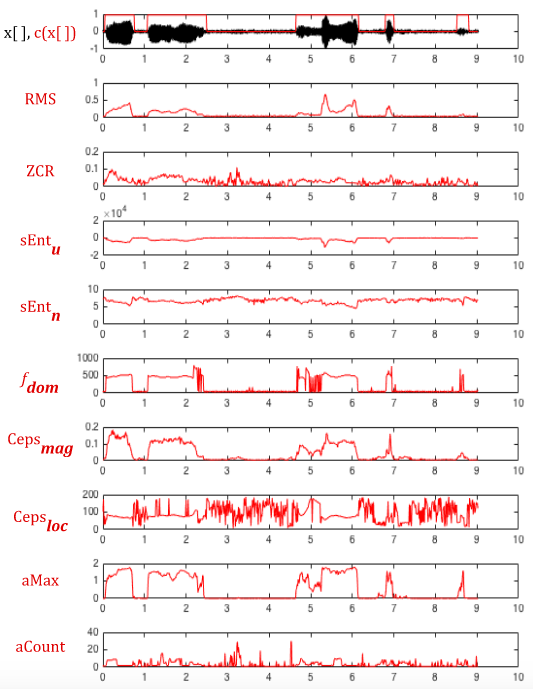
\includegraphics[width=1\textwidth]{bilder/allFeatures01.png}
	\caption{Übersicht über alle Features, die für die Voice Activity Detection erprobt wurden.}
	\label{img:vadAllFeatures}
\end{figure}

\subsubsection{Konstruktion des Feature-Raumes}
\label{sec:theFeatureSpace}

Abbildung \ref{img:min-signal} zeigt in (A) des zeitlichen Verlauf des \emph{RMS}-Attributes eines Signals mit einem Signal/Rauschabstand von \SI{50}{\decibel}. Die Zeiträume mit Stille haben einen weitaus niedrigeren RMS-Wert als die Zeiträume mit Stimme. In (B) ist das selbe Signal mit einem Signal/Rauschabstand von \SI{3}{\decibel} zu sehen. Nun liegen die RMS-Werte der stimmlosen Bereiche nur noch knapp unter denen des Sprachsignals. Zu sehen ist, dass starkes Hintergrundrauschen ähnlich hohe Feature-Werte erzeugen kann wie die Stimme.

\begin{figure}[h]
	\centering
	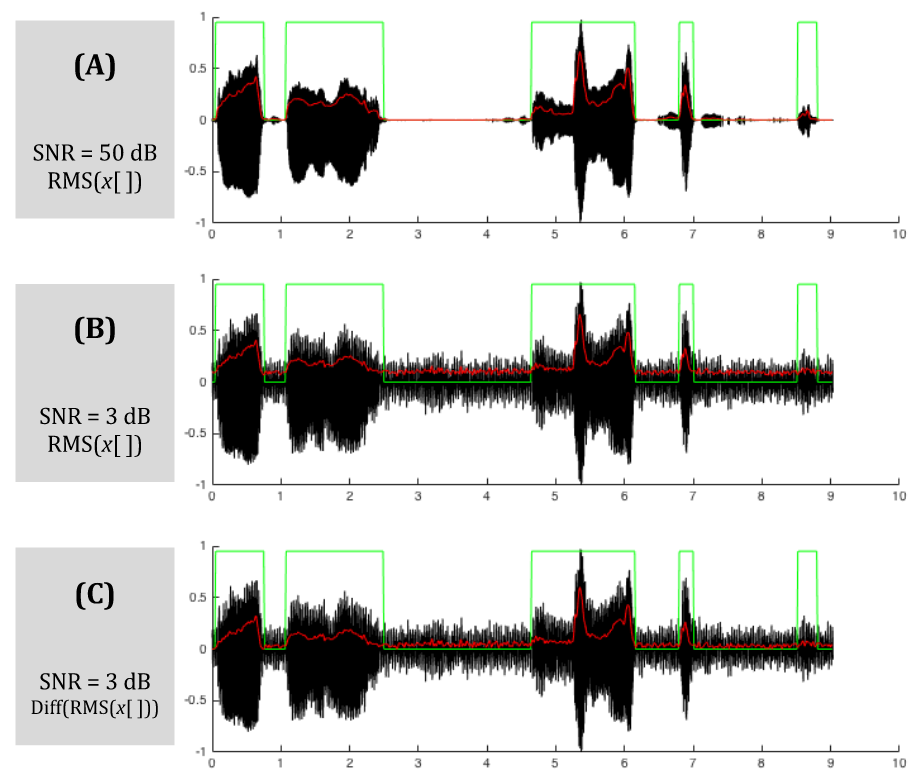
\includegraphics[width=0.7\textwidth]{bilder/rms_diff.png}
	\caption{Das RMS-Feature bei verschiedenen Signal/Rausch-Abständen. Schwarz: Eingangs-Signal $x[\;]$. Grün: Klassifizierung in Stimmhaft/Stille. Rot: Feature-Wert.}
	\label{img:min-signal}
\end{figure}

Moattar et al \cite{vad_Easy} und Waheed et al \cite{vad_entropy} präsentierten die Idee, den Wert des jeweiligen Attributes zu messen, der in den stimmlosen Bereichen durch das Hintergrundrauschen erzeugt wird. Es kann davon ausgegangen werden, dass die ersten Signalfenster eines Signals zunächst noch keine Stimme enthalten, und der Feature-Wert des Rauschens somit anhand dieser Fenster bestimmt werden kann. Bei einer langanhaltenden und kontinuierlichen Analyse können sich sowohl die Signal/Rauschabstände als auch die Qualität des Rauschens ständig ändern, weshalb die von den stimmlosen Bereichen erzeugten Attributwerte regelmäßig aktualisiert werden müssen. Es kann weiterhin davon ausgegangen werden, dass die Länge einer Cry-Unit eine bestimmte Länge $t_{max}$ nicht überschreiten kann, bevor das Baby Luft holen muss und somit ein Zeitfenster mit Stille entsteht. Zeskind et al. \cite[S. 325]{rythmic} haben diesen Wert mit $t_{max} = \SI{4.75}{\second}$ bestimmt. In einem Zeitbereich $ t > t_{max}$ muss somit zumindest ein Feature-Wert enthalten sein, der durch stimmlose Signalteile erzeugt wird. Auf Basis dieser Überlegung wird das \emph{Differenz-Feature} Diff\textsubscript{t}(Feat$(x_i[\;])$) nach Formel \ref{eq:difFeature} definiert als die Differenz zwischen dem aktuell gemessenen Attributwerte und dem geringsten Attributwerte, welcher im vergangenen Zeitbereich $t$ gemessen wurde. Feat$(x_i[\;])$ bezeichnet dabei einen beliebigen Feature-Wert des Signalfensters $x_i[\;]$, $t_{xi}$ die Länge eines Signalfensters in Sekunden (in diesem Fall \SI{25}{\milli\second}), und $t$ der in der Vergangenheit zu durchsuchende Zeitbereich in Sekunden $> t_{max}$. In Abbildung \ref{img:min-signal} wird in (C) das Differenz-Feature für den RMS-Wertes gezeigt.

\begin{equation}
\text{Diff}_t(\text{Feat}(x_i[\;])) = Feat(x_i[\;])\ - \mini_{k=i-z...i}\{Feat(x_k[\;])\}, \qquad z = \frac{2 \cdot t}{t_{xi}}
\label{eq:difFeature}
\end{equation}

Der Feature-Raum wurde schlussendlich folgendermaßen zusammengesetzt: Die ersten 9 Features bildeten die in Attribute \emph{RMS, ZCR, SEnt\textsubscript{u}, SEnt\textsubscript{n}, $f_{dom}$, Ceps\textsubscript{mag}, Ceps\textsubscript{loc}, aMax} und \emph{aCount}. Weiterhin wurde für jedes Attribut nach Formel \ref{eq:difFeature} das Differenz-Feature mit $t = \SI{5}{\second}$ berechnet. Die Features \emph{ZCR, SEnt\textsubscript{u}} und \emph{aCount} wurden vor der Berechnung des Differenz-Features bezüglich ihres Vorzeichens invertiert, da bei Ihnen ein niedriger anstatt ein hoher Wert stimmhafte Signale anzeigen. Das einzige Attribut, für den kein Differenz-Feature berechnet wurde, ist das \emph{Ceps\textsubscript{loc}}-Attribut, da es bei Stille sowohl einen höheren als auch einen niedrigeren Wert annehmen kann. Der Feature-Raum umfasste somit insgesamt $9 + 8 = 17 $ Dimensionen. Gleichung \ref{eq:featureVektor} verdeutlicht die Zusammensetzung des Feature-Vektors $v_i$, der für das Signalfenster $x_i[\;]$ berechnet wurde.

\begin{equation}
v_i = \Big( \text{RMS}(x_i[\;]), ...,\text{ aCount}(x_i[\;]), 
\text{Diff}_{t}(\text{RMS}(x_i[\;])) .... \text{Diff}_{t}(-\text{ aCount}(x_i[\;]))\Big)
\label{eq:featureVektor}
\end{equation}

\subsection{Thresholding}
\label{sec:vad_thresholding}

\subsubsection{Finden der Grenzwerte}

Das Ziel war es nun, Grenzwerte für die Attribute zu finden, bei deren Über- oder Unterschreitung das jeweilige  Signalfenster als \emph{stimmhaft} klassifiziert wird. Abbildung \ref{img:thresholded} verdeutlicht das Prinzip für das \emph{RMS}-Attribut. Diese Entscheidung nach einem Grenzwert ist ein klassisches Vorgehen bei der Voice-Activity-Detection. Eine binäre Klassifizierung nach dem Muster $C(x_i[\;]) = \{ 1, \text{wenn } \text{RMS}(x_i[\;]) \geq 0.18 ,\quad 0 \text{ sonst}\}$ würde in diesem Fall eine weitestgehend richtige Klassifizierung vornehmen.

\begin{figure}[h]
	\centering
	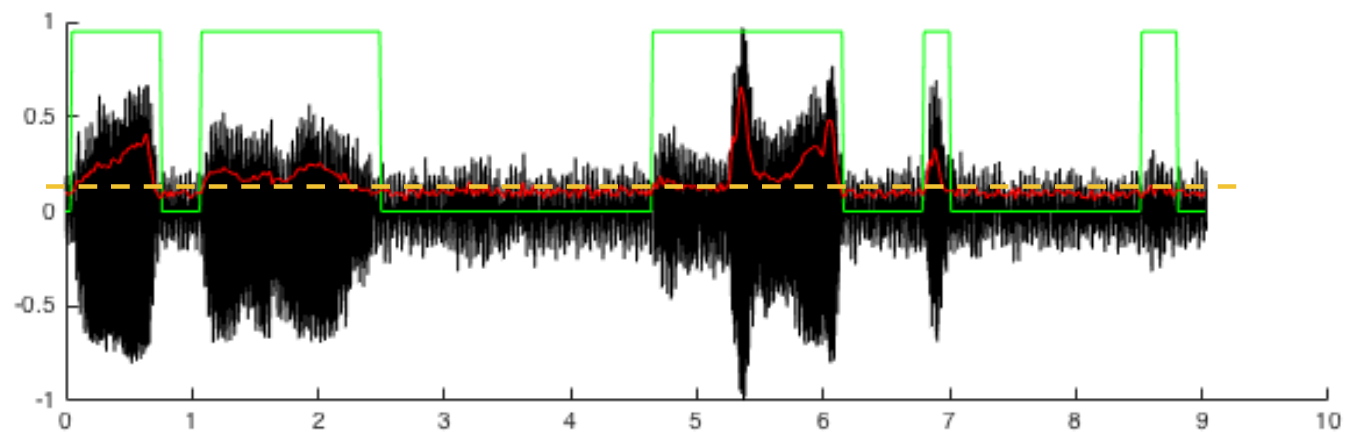
\includegraphics[width=0.6\textwidth]{bilder/thresholded02.png}
	\caption{Thresholding eines Features. Schwarz: Das Eingangssignal $x[\;]$. Grün: Klassifizierung in Stimmhaft/Stille. Rot: RMS-Feature. Orange: Grenzwert}
	\label{img:thresholded}
\end{figure}

Eine Methode zum Finden der optimalen Grenzwerte ist der in Kapitel \ref{sec:c45} vorgestellte \emph{C4.5}-Algorithmus. Da der \emph{C4.5}-Algorithmus Entscheidungsbäume erstellt, kann die Entscheidung über das Vorhandensein von Stimme in einem Signalfenster aufgrund der Verkettung von Grenzwerten mehrerer Attribute in Folge gefällt werden. Ein Beispiel wird in Listing \ref{lst:tree01} dargestellt, bei dem die Klasse eines  Signalfensters hierarchisch zuerst nach einem Grenzwert für Ceps$_{mag}$ und danach für den RMS-Wert entschieden wird.

\begin{lstlisting}[frame=single,mathescape=true,basicstyle=\footnotesize,language=Java,label=lst:tree01,caption=Beispiel eines CART-Entscheidungsbaums,linewidth=1\textwidth]
if Ceps$_{mag}$($x_i[\;]$) > 0.2
|   if RMS($x_i[\;]$) < 0.13
|   |   C($x_i[\;]$) = 0
|   |else
|   |   C($x_i[\;]$) = 1
|else
|    C($x_i[\;]$) = 1
\end{lstlisting}

\subsubsection{Trainings- und Testdatensätze}
\label{sec:databases}

Es wurden sechs Audioaufnahmen mit Weinen verschiedener Babies von der freien Online-Sound-Bibliothek \url{https://www.freesound.org/} heruntergeladen und zu Segmenten \`{a} \SI{10}{\second} beschnitten. Es handelt sich um weitgesgehend rauschfreie Aufnahmen, die von verschiedenen Babys stammen. In den Audiosignalen wurden manuell die Zeitbereiche markiert, welche Stimme enthalten. Es wurden \emph{keine} Geräusche markiert, bei denen es sich offensichtlich um Einatumungs-Geräusche handelt. Geräusche, bei denen nur Anhand der Aufnahme nicht mit Sicherheit festgestellt werden konnte, ob es sich um Einatmungs- oder Ausatmungsgeräusche handelt, wurden als Stimme markiert. Weiterhin wurden drei verschiedene Rauschsignale heruntergeladen. Es handelt sich um \glqq realistische\grqq{} Atmosphären von Krankenhäusern. Jedes der sechs Audioaufnahmen der Babys wurde mit jedem der drei Rauschsignale überlagert, einmal mit einem Signal/Rausch-Abstand von \SI{50}{\decibel} (\glqq fast unhörbares Rauschen\grqq), und einmal mit einem Signal/Rausch-Abstand von \SI{3}{\decibel} (\glqq starkes Rauschen\grqq). Außerdem wurde ein siebte Aufnahme eines Babys heruntergeladen, welches mit einem vierten Rauschsignal mit einem SNR von \SI{7}{\decibel} überlagert wurde. Dieses Signal spielt eine Sonderrolle, da es nur zur Verifikation verwendet wird. So wurden vier Mengen an Audiosignalen erzeugt:

\begin{description}
	\item[A\textsubscript{\SI{50}{\decibel}}] enthält $3 \cdot 6 = 18$ Audiosignale, bei dem alle sechs Baby-Aufnahmen mit den drei Rauschsignalen bei einem Signal/Rausch-Abstand von \textbf{\SI{50}{\decibel}} überlagert wurden
	
	\item[A\textsubscript{\SI{3}{\decibel}}] enthält $3 \cdot 6 = 18$ Audiosignale, bei dem alle sechs Aufnahmen der Babys mit den drei Rauschsignalen bei einem Signal/Rausch-Abstand von \textbf{\SI{3}{\decibel}} überlagert wurden
	
	\item[A\textsubscript{50+\SI{3}{\decibel}}] $ = \{ A_{\SI{50}{\decibel}} \cup  A_{\SI{3}{\decibel}}\} = 32$ Audiosignale
	
	\item[A\textsubscript{\SI{7}{\decibel}*}] enthält $1$ Audiosignal, bei dem eine siebte Aufnahme eines Babys mit einem vierten Rauschsignal bei einem Signal/Rausch-Abstand von \textbf{\SI{7}{\decibel}} überlagert wurde
	
\end{description}

Im nächsten Schritt werden die eigentlichen Datensätze $D_{SNR,Feats}$ gebildet, in dem Audiosignale dieser Signalmengen (1) wie in Kapitel \ref{sec:preprocessing} beschrieben vorverarbeitet werden, (2) wie in Kapitel \ref{sec:windowing} in die Signalfenster \`{a} \SI{25}{\milli\second} zerlegt werden und (3) für jedes Signalfenster der durch Gleichung \ref{eq:featureVektor} definierte Featurevektoren berechnet wird. Außerdem wird jedem Featurevektor die Klasseninformation \emph{Stimme/Stille} zugewiesen.

Es ist rechnerisch zu aufwendig, alle genannten Features in einem kontinuierlichen System zur Voice Activity Detection zu berechnen. Daher werden die Datensätze in Untermengen bezüglich der verwendeten Features eingeteilt. Das Ziel ist es, eine möglichst kleine Untermenge an Features zu finden, die sich am besten für die Voice Activity Detection sowohl bei niedrigem als auch bei starkem Hintergrundrauschen eignet. Die Untermengen werden in Bezug auf die Methode gebildet, durch die die Features berechnet werden. Das heißt, dass beispielsweise die Untermenge \emph{Zeit} die in Kapitel \ref{sec:timeFeats} beschriebenen Features \emph{RMS} und \emph{ZCR} sowie die dazugehören Differenzfeatures \emph{Diff\textsubscript{t}(RMS)} und \emph{Diff\textsubscript{t}(ZCR)} beinhaltet. 

Die 9 Untermengen sind: \{ Zeitbereich, Frequenzbereich, Cepstrum, Autokorrelation, Zeit + Frequenzbereich, Zeit + Cepstrum, Zeit + Autokorrelation, Frequenzbereich + Cepstrum, Frequenzbereich + Autokorrelation \}. Cepstrum- und Autokorrelation werden nicht gemeinsam in eine Untermenge hinzugefügt, da sie in Bezug auf den Berechnungsaufwand die aufwendigsten sind. So enthält beispielsweise der Datensatz $D_{\SI{3}{\decibel},Zeit}$ die Featurevektoren des Zeitbereiches für die Audiosignale mit einem Signal-Rausch-Abstand von \SI{3}{\decibel}. Alle Audiosignal-Mengen [A\textsubscript{\SI{50}{\decibel}}], [A\textsubscript{\SI{3}{\decibel}}], [A\textsubscript{50+\SI{3}{\decibel}}] und [A\textsubscript{\SI{7}{\decibel}}] wurden in Datensätze umgewandelt. Es wurden schlussendlich $4 \cdot 9 = 36$ Datensätze gebildet.

\subsubsection{Training} 
\label{sec:training}

Das Ziel ist, mit Hilfe des \emph{C4.5}-Algorithmus einen Entschidungsbaum zu finden, der auf Basis einer möglichst geringen Feature-Menge eine möglichst hohe Klassifkationsgenauigkeit für sowohl niedrige als auch hohe Signal/Rausch-Abstänge erzielt. Die Frage ist, ob ein Entschiedungsbaum, der auf Basis von Signalen mit niedrigem SNR gebildet wird, auch für hohe SNRs eine hohe Klassifikationsgenauigkeiten erzielt, oder ob der umgedrehte Fall zutreffend ist. Daher werden die Entscheidungsbäume sowohl auf Basis verschiedener SNRs als auch verschiedener Feature-Untermengen gebildet. Die Entschäudungsbäume werden daraufhin gegen die Signale mit den verschiedenen SNRs evaluiert. Wird also beispielsweise der Datensatz $D_{\SI{50}{\decibel},Zeit}$ zum Training und der Datensatz $D_{\SI{3}{\decibel}}$ zum Testing verwendet, so wird berechnet, wie gut sich der Klassifikator unter Verwendung der Zeit-Features zur Klassifizierung niedriger SNRs eignet, obwohl er für hohe SNRs entworfen wurde. Dabei ist unerheblich, welche Features der Test-Datensatz verwendet, da bei der Evaluation nur die Klasseninformation der Instanzen verwendet werden.

Die Implementierung, die für den \emph{C4.5}-Algorithmus verwendet wurde, ist der \emph{REPTree} \footnote{Dokumentation von REPTree: \url{http://weka.sourceforge.net/doc.dev/weka/classifiers/trees/REPTree.html}} der Open Source Data-Mining-Bibliothek \emph{Weka}\footnote{Download von WEKA: \url{http://www.cs.waikato.ac.nz/ml/weka/}}. Die Implementierung hat den Vorteil, dass die maximale Tiefe des Entscheidungsbaumes festlegbar ist und somit die Komplexität des Baumes begrenzt werden kann, um Overfitting zu vermeiden.

Es wurden insgesamt $3 \cdot 9 = 27$ Trainings-Datensätze erzeugt ( [3 SNR-Werte: \SI{3}{\decibel}, \SI{50}{\decibel} und 50+\SI{3}{\decibel} ] $\times$ [9 Feature-Untermengen]. Der Datensatz mit einem SNR von \SI{7}{\decibel} wurde \emph{nicht} zum Training verwendet). Mit diesen 27 Trainingsdatensätze wurden mit Hilfe des \emph{REPTree}-Algorithmus 27 Klassifikationsbäume erzeugt. Jeder Klassifikationsbaum wurde gegen die 3 Testdatensätze D\textsubscript{\SI{3}{\decibel}}, D\textsubscript{\SI{50}{\decibel}} und D\textsubscript{\SI{7}{\decibel}*} evaluiert und die Accuracy berechnet. Das Signal A\textsubscript{\SI{7}{\decibel}*} erfüllt dabei eine Sonderrolle, da es nicht in den Trainingsdatenstäzen enthalten ist und somit der Kontrolle bezüglich Overfitting dient. Da jeder Datensatz ungefähr dreimal so viele stimmhafte Examples wie nicht-stimmhafte enhthielt, wurde jede stimmlose Instanz eines Datensatzes dreimal eingefügt. Somit wurde in jedem Datensatz  ein ausgewogenes Verhältnis zwischen positiven und negativen Examples gewährleistet. Um die Komplexitiät des Entscheidungsbaumes zu verringern eine Nutzung von möglichst wenig Features zur Klassifizierung zu erzwingen, wurde die maximale Tiefe des REPTree auf 2 gesetzt. 

\subsubsection{Ergebnis} 
\label{sec:vad_result}

Die Evaluations-Ergebnisse  sind in Tabelle \ref{tab:reptree_results} zu sehen. Für jeden Trainingsdatensatz mit einem bestimmten SNR und einer Feature-Untermenge wird die Accuracy für den jeweilgen Test-Datensatz mit einem SNR von \SI{3}{\decibel}, \SI{50}{\decibel} und \SI{7}{\decibel}* angegeben.\footnote{Der Stern verdeutlicht die Sonderrolle des  Datensatzes mit einem SNR von \SI{7}{\decibel}, da er nur zu Evaluation verwendet wurde}. Außerdem wird der Durchschnittswert aller drei jeweiligen Accuracy-Werte angegeben.

Die Features, welche zu den höchsten Accuracy-Werten führten, sind die des \emph{Cepstrum}-Bereiches, genauer gesagt das Diff\textsubscript{t}(Ceps\textsubscript{mag})-Feature, da es vom REPTree als einziges Feature dieses Bereiches für die Entscheidungsbäume ausgewählt wurde. Die Entscheidungsbäume, die mit dem Diff\textsubscript{t}(Ceps\textsubscript{mag})-Feature entworfen wurden, erreichten eine durchschnittliche Accuracy von mindestens 91,45\%. Der nächstbeste Klassifikator mit einer Accuracy von 86,96\% wurde unter Verwendung der Features des Zeitbereiches und der Autokorrelation auf dem Datensatz D\textsubscript{50+\SI{3}{\decibel},Zeit+Correlation} entworfen. Sobald die Cepstrum-Features in Verbindung mit den Features anderer Bereiche verwendet wurden, wurde das Diff\textsubscript{t}(Ceps\textsubscript{mag})-Feature vom REPTree-Algorithmus bevorzugt und die Features der anderen Bereiche nicht mehr verwendet.

Auf Basis der Datensätze D\textsubscript{\SI{3}{\decibel},Ceps}, D\textsubscript{\SI{3}{\decibel},Zeit+Ceps}, D\textsubscript{\SI{3}{\decibel},Freq+Ceps}, D\textsubscript{50+\SI{3}{\decibel},Ceps}, \\ D\textsubscript{50+\SI{3}{\decibel},Zeit+Ceps} sowie D\textsubscript{50+\SI{3}{\decibel},Freq+Ceps} wurde der selbe Klassifikator erzeugt, der in Gleichung \ref{eq:cepTree01} definiert wird. Wie zu sehen ist, handelt es sich um einen einfachen Grenzwert des \emph{v.Diff\textsubscript{t}(Ceps\textsubscript{mag})}-Features, da trotz der höchst möglichen Baumtiefe von 2 nur eine Tiefe von 1 genutzt wurde.

\begin{equation}
C(v) = \begin{cases}
1, \quad \text{if } v.Diff_t(Ceps_{mag}) > 0.02, \\
0 \quad \text{else}
\end{cases}
\label{eq:cepTree01}
\end{equation}


Auf Basis der Datensätze D\textsubscript{\SI{50}{\decibel},Ceps} und D\textsubscript{\SI{50}{\decibel},Zeit+Ceps} wurde der Klassifikator nach Gleichung \ref{eq:cepTree02} erzeugt. Er unterscheidet sich von dem Klassifikator aus Gleichung \ref{eq:cepTree01} nur durch den Grenzwert.

\begin{equation}
C(v) = \begin{cases}
1, \quad \text{if } v.Diff_t(Ceps_{mag}) > 0.03, \\
0 \quad \text{else}
\end{cases}
\label{eq:cepTree02}
\end{equation}

Da der Klassifikator aus Gleichung \ref{eq:cepTree01} eine durchschnittliche Accuracy von 92,22\% und der Klassifikator aus Gleichung \ref{eq:cepTree02} eine unwesentlich geringere Accuracy von 91,45\% erzielt, wurden für beide Modelle die Specificity und Sensitivity berechnet, um eine Entscheidung für eines der beiden Modelle fällen zu können. Dazu wurden die Signalmengen A\textsubscript{\SI{3}{\decibel}}, A\textsubscript{\SI{50}{\decibel}} und A\textsubscript{\SI{7}{\decibel}*} in Frames \`{a} 100 Windows zerlegt und für jedes Zeitfenster die Senstivity, Specificity und Accuracy bezüglich der beiden Klassifikatoren berechnet. Die Ergebnisse werden als Boxplots in Abbildung \ref{img:boxplots} dargestellt. Die Modelle unterscheiden sich am stärksten hinsichtlich der Datensätze mit \SI{3}{\decibel} und \SI{7}{\decibel}. Der Klassifikator mit dem Grenzwert von 0.03 erzielt in beiden Fällen eine höhere Specificity, aber geringere Senstivitiy als das Modell mit dem Grenzwert von 0.02. Es wurde sich für das Modell für mit einem Grenzwert von 0.02 entschieden, da durch die höhere Senstivity mehr Cry-Units erkannt werden, die in späteren Verarbeitungsschritten immernoch als False-Positives erkannt und verworfen werden können. Einmal im Prozess der VAD als Stimmlos markierte Fenster werden jedoch nicht weiter verarbeitet und gehen somit \glqq verloren\grqq. 

Die finale Klassifikations-Funktion eines Signalfensters $C(x_i[\;]) \mapsto \{ 0 \hat{=} \text{Stille}, 1 \hat{=} \text{Stimme}\}$ wird somit durch Gleichung \ref{eq:vad-final} gegeben, wobei $c_i[\;]$ das Cepstrum des Signalfensters ist.

\begin{equation}
C(x_i[\;]) = \begin{cases}
1, \quad \text{if } v.Diff_t(Ceps_{mag}(c_i[\;])) > 0.02, \\
0 \quad \text{else}
\end{cases}
\label{eq:vad-final}
\end{equation}

\subsection{Markierung der Cry-Units}
\label{sec:CryUnit}

Wird die Voice-Activity-Detection für das Signal $x[\;]$ nach Gleichung \ref{eq:vad-final} durchgeführt, ist das Ergebnis eine Zuordnung der Signalfenster $x_0[\;] \ldots x_m[\;]$ zu den Klassen Stimme/Stille. Varallyay \cite[S. 16 - 17]{cry_thesis} stellt die Idee vor, auf Grundlage der Informationen der Voice-Activity-Detection die Anfangs- und Endzeitpunkte der Cry-Units zu markieren (welche er als Cry-Segmente beschreibt). Das genaue Vorgehen konnte jedoch nicht eingesehen werden, da der Autor keine Zugriffsrechte auf die Publikation erhielt.

Waheed et al \cite{vad_entropy} stellen die Idee vor, zusammenhängende und ununterbrochene Ketten als \emph{stimmhaft} klassifizierter Signalfenster zu \emph{Stimm-Segmenten} zusammenzufassen. Dieser Ansatz wird übernommen, wobei ein Stimmsegment im Kontext dieser Arbeit einer \emph{Cry-Units} entspricht. Möglicherweise ist dies der Ansatz, den auch  Varallyay \cite[S. 16 - 17]{cry_thesis} gewählt hat. Abbildung \ref{img:cryUnit} veranschaulicht diese Gruppierung. 

\begin{figure}[h]
	\centering
	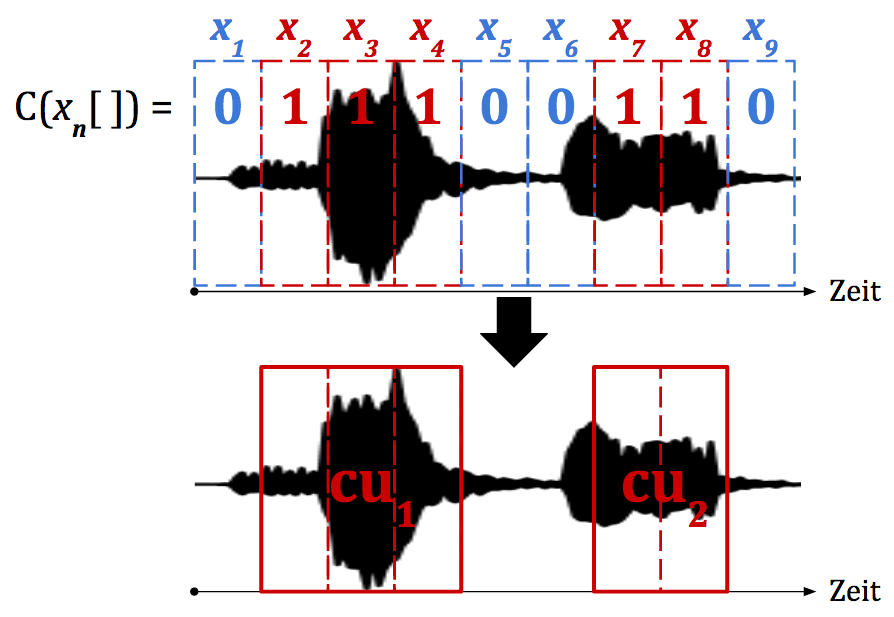
\includegraphics[width=0.6\textwidth]{bilder/cry-Unit02.png}
	\caption{Zusammenfassung klassifizierter Signalfenster zu Cry-Units}
	\label{img:cryUnit}
\end{figure}

Formel \ref{eq:cry-Unit} gibt die Definition des Datentypes \emph{Cry-Unit} [$CU$]. Eine Cry-Unit wird definiert durch den Anfangszeitpunkt $start$, einen Endzeitpunkt $end$ und der Liste seiner Signalfenster $windows = [x_0[\;], \ldots, x_n][\;]$.

\begin{equation}
CU = (windows = \big[x_0[\;] ,\ldots, x_n[\;] \big], start \in Zeit, end \in Zeit)
\label{eq:cry-Unit}
\end{equation}

Die Dauer eine Cry-Unit $cu \in CU$ wird nach Formel \ref{eq:cry-Lambda} berechnet und mit $\lambda$ bezeichnet. Die zeitliche Dauer der Pause zwischen zwei Cry-Units d($cu_i, cu_j$), wird nach Formel \ref{eq:cry-distance} berechnet. Diese Zusammenhänge werden in Abbildung \ref{img:cryUnit-details} visualisiert.\cite[S. 2]{vad_entropy}

\begin{equation}
\lambda (cu) = cu.end - cu.start
\label{eq:cry-Lambda}
\end{equation}

\begin{equation}
\text{d}(cu_i, cu_j) = cu_j.start - cu_i.end
\label{eq:cry-distance}
\end{equation}

\begin{figure}[h]
	\centering
	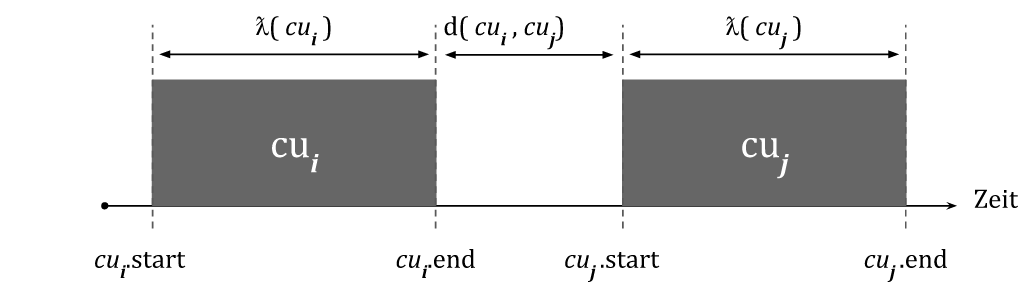
\includegraphics[width=0.8\textwidth]{bilder/newSmoothing05.png}
	\caption{Beziehung zwischen agrenzenden Cry-Units, nach \cite[S. 2]{vad_entropy}}
	\label{img:cryUnit-details}
\end{figure}

Algorithmus \ref{alg:cryUnit} zeigt in Pseudo-Code, wie auf Basis der Liste aller Signalfenster eines Signals $X_{all} = [x_0[\;] ,\ldots, x_m[\;]]$ die Liste der Cry-Units $CU_{all}$ generiert wird. Die Funktion $C(x[\;])$ ist die Klassifikations-Funktion der Signalfenster in Stille/Stimme nach Gleichung \ref{eq:vad-final}. Die Funktion getTimeOf$(x_i[\;])$ liefert die Anfangszeitpunkt des Signalfensters $x_i[\;]$.

\begin{algorithm}[h]
	\caption{Gruppierung von Signalfenstern zu Cry-Units}
	\label{alg:cryUnit}
	\begin{algorithmic}[1]
		\Function{turnWindowsIntoCryUnits}{$X_{all}$}
		\State $ CU_{all} \gets [\;]$
		\State $ cu\gets ([\;],0,0)$
		\For{\textbf{all} $x_i[\;] \in X_{all}$}
				\State $ c \gets C(x_i[\;])$
				\State \Comment Start of Cry-Unit
				\If {$c == 1 \wedge \text{isEmpty}(cu.windows)$}
						\State $cu\gets ([\;],0,0)$
						\State $cu.start \gets \text{getTimeOf}(x_i[\;])$
						\State $cu.windows \gets [cu.windows, x_i[\;]]$
				\EndIf
				\State \Comment Inside Cry-Unit
				\If {$c == 1 \wedge \text{ ! isEmpty}(cu.windows)$}
						\State $cu.windows \gets [cu.windows, x_i[\;]]$
				\EndIf
				\State \Comment End of Cry-Unit
				\If {$c == 0 \wedge \text{ ! isEmpty}(cu.windows)$}
						\State $cu.end \gets  getTimeOf(x_i[\;])$
						\State $CU \gets [CU, cu]$
						\State $cu.windows \gets [\;]$
				\EndIf
		\EndFor
		
		\State \Comment End last Cry-Unit by force if still open.
		\If {$\text{ ! isEmpty}(cu.windows) == 0$}
		\State $cu.end \gets  getTimeOf(X_{windows}[end])$
		\State $CU_{all} \gets [CU_{all}, cu]$
		\EndIf
		
		\Return $CU_{all}$
		
		\EndFunction
		
	\end{algorithmic}
\end{algorithm}

\subsection{Decision Smoothing}
\label{sec:smoothing}

Abbildung \ref{img:beforeSmoothing} zeigt ein Audiosignal mit einem Signal-Rausch-Abstand von \SI{3}{\decibel}, bei dem die Voice Activity Detection durchgeführt wurde. Die rote Linie zeigt die tatsächliche Klassifiikation und die grüne Linie die prognostizierte Klassifikation. Es ist zu sehen, dass einige False-Negatives und prongnostiziert wurden. Im folgenden werden drei charakteristische Arten falscher Klassifikationen näher erläutert:

\begin{description}
	\item [False Negatives nach (a): ] Eine korrekt erkannte, längere Cry-Unit wird zu früh beendet. Oft werden kurz nach dem Ende einer längeren Cry-Unit sehr kurze Cry-Units erkannt, die eigentlich noch zu der längeren, vorhergehenden Cry-Unit gehören.
	\item [False Positives nach (b): ] Kurze Cry-Units werden in eigentlichen Stille-Bereichen erkannt.
	\item [False Negatives nach (c): ] Eine Cry-Unit zerfällt in zwei Cry-Units, da kurze Signalfenster in der Mitte als Stille erkannt wurden.
\end{description}

\begin{figure}[h]
	\centering
	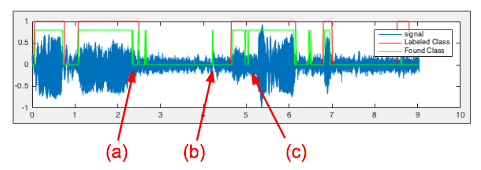
\includegraphics[width=0.7\textwidth]{bilder/smoothing02.png}
	\caption{Klassifizierung vor dem Decision Smoothing}
	\label{img:beforeSmoothing}
\end{figure}

Im Process des \textbf{Decision Smoothing} werden kontextuelle Informationen genutzt, um nachträglich False-Positives und False-Negatives zu entfernen. Es werden dazu die von Waheed et al \cite{vad_entropy} präsentierten Ideen verwendet. Es werden zwei Parameter eingeführt: $\lambda_{min}$, die Mindestlänge einer akzeptierten Cry-Unit, und d$_{min}$, die Mindestlänge eines akzeptierten Stille-Segmentes. Das Decision-Smoothing wird nach den folgenden Entscheidungsregeln durchgeführt:

\pagebreak
\noindent\rule{\linewidth}{0.3pt}
\begin{itemize}
	\item ist $\lambda (cu_{i}) \leq \lambda_{min}$ ?
	\begin{itemize}
		\item wenn $\lambda (cu_{i-1}) > \lambda_{min}$ und $d (cu_{i-1}, cu_{i}) \leq d_{min}$, dann vereinige $cu_{i}$ mit $cu_{i-1}$ . $\Longrightarrow$ behebt False-Negatives des Types (a)
		\item ansonsten entferne $cu_i \Longrightarrow$ behebt False-Negatives des Types (b)
	\end{itemize}
	\item wenn $\lambda (cu_{i}) > \lambda_{min}$ und $d (cu_{i-1}, cu_{i}) \leq d_{min}$, dann vereinige $cu_{i}$ mit $cu_{i-1}$ . $\Rightarrow$ behebt False-Negatives des Types (c)
\end{itemize}
\noindent\rule{\linewidth}{0.3pt}

Die Entscheidungsregeln greifen nur auf die letzten beiden erkannten Cry-Units zu, um eine kontinuierliche Analyse zu gewährleisten. Bei einer kontinuierlichen Analyse wird die Auswertung um die Zeitdauer einer Cry-Unit verzögert, da die Entscheidungsregeln erst nach Beendigung einer Cry-Unit abgefragt werden können. Bei einer offline-Analyse können die Entscheidungsregeln vereinfacht werden, da die False-Negatives nach Typ (a) und (c) mit der selben Regel abgefragt werden können. Algorithmus \ref{alg:decisionSmoothing} zeigt in Pseudo-Code, wie das Decision-Smoothing durchgeführt wird. Input der Funktion ist die Liste aller Cry-Units $CU_{all} = [cu_0 , \ldots , cu_n]$, die durch Algorithmus \ref{alg:cryUnit} entstanden ist, sowie die Grenzwerte $\lambda_{min}, d_{min}$. Der Output der Funktion ist die Liste aller Cry-Units nach dem Decision-Smoothing $CU_{smoothed}$.

\begin{algorithm}[h]
	\caption{Decision-Smoothing for VAD}
	\label{alg:decisionSmoothing}
	\begin{algorithmic}[1]
		\Function{decisionSmoothing}{$CU_{all}, \lambda_{min}, d_{min}$}
		\State $CU_{smoothed} \gets[CU_{all}[0]] $
		\State \Comment start for-loop at the \emph{second} cry-Unit!
		\For{ $i = 1 , \ldots , length(CU_{all}) - 1$}
			\State $cu_i \gets CU_{all}[i]$
			\State $cu_{i-1} \gets CU_{smoothed}[end]$
			\If{$\lambda(cu_i) > \lambda_{min}$}
			\State \Comment Accept Cry-Unit
			\If{d$(cu_{i-1},cu_{i}) > d_{min}$}
					\State $CU_{smoothed} \gets [CU_{smoothed}, cu_i] $
			\Else
					\State \Comment Erase False-Negative Type (c)
					\State $cu_i \gets \text{vereinige}(cu_i, cu_{i-1})$
					\State $CU_{smoothed} \gets [CU_{smoothed}[1:end-1], cu_i] $
			\EndIf
			\Else
			\State \Comment Erase False-Negative Type (a)
			\If{$d(cu_{i-1},cu_{i}) \leq d_{min}$ }
			\State $cu_i \gets \text{vereinige}(cu_i, cu_{i-1})$
			\State $CU_{smoothed} \gets [CU_{smoothed}[0:end-1], cu_i] $
			\Else
			\State \Comment Don't accept $cu_i$. Erases False-Positives (b)
			\EndIf
			\EndIf
		\EndFor
		
		\Return $CU_{smoothed}$
		\EndFunction
		
	\end{algorithmic}
\end{algorithm}

Abbildung \ref{img:after-smoothing} zeigt das Beispielsignal vor und nach dem Decision-Smoothing. In verschiedenen Veröffentlichungen wurden unterschiedliche Mindestlängen von Cry-Units festgestellt. Varallyay \cite[S. 8]{cry_thesis} hat beispielsweise eine Mindestlänge von \SI{250}{\milli\second} gemessen. Der geringste Wert, der nach dem Wissen des Autors in einer Veröffentlichung genannt wurde, stammt von Zeskind et al \cite[S. 325]{rythmic} und beträgt  \SI{60}{\milli\second}, welcher für $\lambda_{min}$ übernommen wurde. Es konnten hingegen keine Werte über die geringste festgestellte Pause zwischen zwei Cry-Units gefunden werden. Der Wert wurde daher auf Basis des verwendeten Trainings-Datensatzes ebenfalls mit $d_{min} = \SI{60}{\milli\second}$ bestimmt. 

\begin{figure}[h]
	\centering
	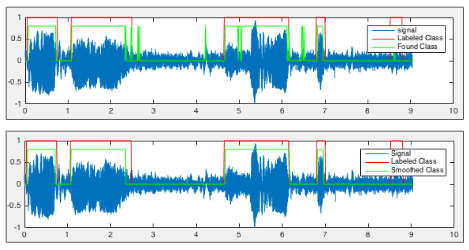
\includegraphics[width=0.6\textwidth]{bilder/smoothing04.png}
	\caption{Klassifikation vor und nach dem Decision Smoothing}
	\label{img:after-smoothing}
\end{figure}

\subsection{Diskussion der Voice-Activity-Detection}

In diesem Kapitel wurden verschiedene Methoden der Voice Activity Detection vorgestellt, verglichen und evaluiert, wobei eine Voice Activity Detection auf Basis des Cepstrums die besten Ergebnisse erzielte. Unabhängig von den konkret verglichenen Features werden in dieser grundlegenden Herangehensweise zur Voice Activity Detection kontextuelle Informationen in Bezug auf den zeitlichen Verlauf der Stimme jedoch nur in einem geringen Maße beim Decision-Smoothing verwertet. Schlussendlich markiert der VAD-Algorithmus eine Reihe von kurzen Signalfenstern genau dann als zusammenhängende Cry-Unit, wenn jedes Signalfenster für sich betrachtet als Lautäußerung eines Babies klassifiziert wurde. Ob jedoch die Reihenfolge der in den Signalfenstern enthaltenen Lautäußerungen Sinn macht, wird nicht betrachtet. Schneidet man beispielsweise wenige Sekunden aus der Mitte einer längeren Cry-Unit aus und konkateniert dieses Sample viele Male, um eine synthetische, längere Cry-Unit zu erzeugen, klingt das Ergebnis für den Menschen stark unnatürlich, wird von dem hier vorgestellten VAD-Algorithmus jedoch trotzdem als valide Cry-Unit markiert. Das Cepstrum als Feature mit der höchsten Accuracy ist somit so zu bewerten, dass es vor allem im geringen Maße kontextuell Informationen benötigt, um eine Entscheidung über das vorahndensein von Stimme zu fällen. Zukünftige Forschungen könnnen an diesem Punkt ansetzen, um die Accuracy der VAD zu erhöhen.

\section{Segmentierung}
\label{sec:segmenting}
Das Ergebnis der Voice-Activiy-Detection ist eine Liste an Cry-Units  $cu_0 \ldots cu_n$. Pain-Scores werden nicht aus einzelnen Cry-Units abgeleitet, sondern aus dem Verbund mehrerer Cry-Units. Daher ist es notwendig, die Cry-Units zu Segmenten zusammenzufassen. Dieser Prozess des Gruppieren von Cry-Units zu Segmenten wird in dieser Arbeit kurz als \emph{Segmentierung} (engl. \emph{Segmenting}) bezeichnet. Die Frage ist, nach welchen Kriterien Cry-Units zu Segmenten zusammengefasst werden. Abbildung \ref{img:segmenting02} verdeutlicht das Problem, in dem drei mögliche Segmentierungen für eine Signal beispielhaft gezeigt werden.

\begin{figure}[H]
	\centering
	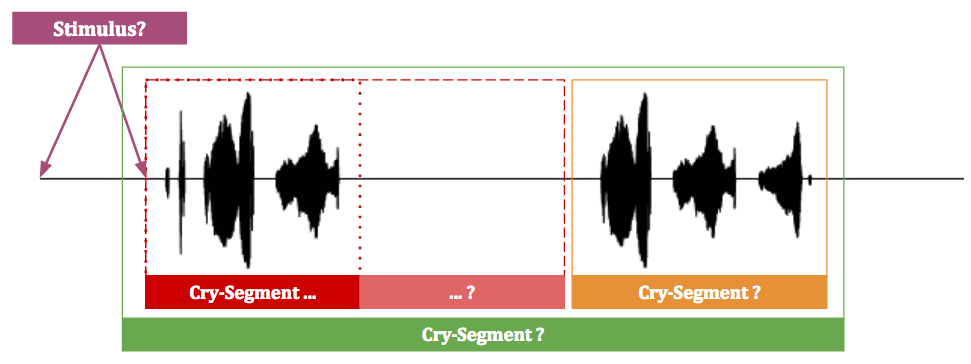
\includegraphics[width=0.7\textwidth]{bilder/segmentierung07.png}
	\caption{Mögliche Segmentierungen eines Signals}
	\label{img:segmenting02}
\end{figure}

Ein Cry(-Segment) wird von Golub et al definiert als \glqq die komplette klangliche Antwort auf einen spezifischen Stimulus. Sie kann mehrere Cry-Units entahlten \grqq. \cite[S. 61, übersetzt aus dem Englischen]{cryModel}. Die Defintion lässt unter Anderem die folgenden Fragen offen:

\begin{itemize}[leftmargin=*]
	\item Beginnt das Segment bereits bei Zuführung des Stimulus, oder erst ab der ersten Cry-Unit? 
	\item Wodurch definiert sich der Beginn, wenn der Stimulus unbekannt ist?
	\item Endet ein Cry-Segment mit Ende der letzten \glqq Cry-Unit\grqq{}, oder erstreckt es sich bis zu Beginn des nächsten Cry-Segmentes?
\end{itemize}

Keines der in Kapitel \ref{sec:system_literature} vorgestellten Veröffentlichungen schlägt Methoden zur Segmentierung vor. Bei den nicht-kontinuierlichen Systemen werden manuell beschnittene Cry-Segmente verwendet. Entweder werden keine objektiv messbaren Krtierien gegeben (außer \grqq das Segment dort zu beenden, wo das Baby aufhört, zu weinen\grqq{}), oder feste Längen wie zum Beispiel \SI{90}{\second}\cite[S. 324]{rythmic} gegeben. Bei den kontinuierlichen Systemen wird die Segmentierung nicht als Verarbeitungsschritt erwähnt, eventuell, weil keine stattfindet.

Es wird daher das folgende Vorgehen zur kontinuierlichen Segmentierung vorgeschlagen: Wenn das Baby keine Äußerungen von sich gibt, weil es beispielsweise schläft, wird keine Cry-Unit festgestellt, und somit existiert auch momentan kein offenes Segment. Fängt das Baby an, einen Laut von sich zu geben, also eine Cry-Unit zu produzieren, wird ein neues Segment eröffnet und die Cry-Unit diesem Segment hinzugefügt. Weitere Cry-Units werden so lange diesem Segment hinzugefügt, wie die Dauer der Stille nach einer Cry-Unit einen festgelegten Grenzwert $t_{s}$ nicht überschreitet. Ein Cry-Segment wird folglich dann geschlossen, wenn das Baby \glqq aufhört, zu weinen\grqq{}, also keine Laute mehr für einen festgelegten Zeitraum von sich gibt. Das Endzeitpunkt des Segmentes wird als der Endzeitpunkt der letzten Cry-Unit des Segmentes festgelegt.

Formel \ref{eq:cry-segment}  definiert ein \emph{Cry-Segment} [$CS$] als Datentyp. Ein Cry-Segment ist eine Liste von Cry-Units. Alle Cry-Units erfüllen die Nebenbedingung \ref{eq:cry-segment-nb}, das heißt, dass die Distanzen aller benachbarter Cry-Units eines Cry-Segments unterhalb des Grenzwertes $t_{s}$ liegen.

\begin{equation}
CS = [cu_0 ,  \ldots,  cu_n]
\label{eq:cry-segment}
\end{equation}

\begin{equation}
\forall cs \in CS: \forall i = 0 \ldots length(cs)-2 : d(cs[i], cs[i+1]) < t_{s}
\label{eq:cry-segment-nb}
\end{equation}

Der Start-Zeitpunkt eines Cry-Segmentes wird nach Formel \ref{eq:cry-segment-start} als der Startzeitpunkt der ersten Cry-Unit des Segmentes definiert. Das Ende eines Segmentes wird definiert als das Ende der letzten Cry-Unit nach Gleichung \ref{eq:cry-segment-end}.

\begin{equation}
start(cs) = cs[0].start
\label{eq:cry-segment-start}
\end{equation}

\begin{equation}
end(cs) = cs[n].end
\label{eq:cry-segment-end}
\end{equation}

Algorithmus \ref{alg:crySegment} zeigt einen Pseudocode, wie die Segmentierung nach dem beschriebenen Prinzipien offline durchgeführt wird. Input des Algorithmus ist die Liste aller Cry-Units $CU_{all} = [cu_0 ,\ldots, cu_m]$, die nach dem Decision-Smoothing nach Algorithmus \ref{alg:decisionSmoothing} entstanden ist.  Das Ergebnis des Algorithmus ist die Liste, die alle gefundene Cry-Segmente  $[cs_0 \ldots  cs_n]$ enthält. Der Algorithmus eignet sich nicht für eine Online-Segmentierung, da das Ende eines Segmentes erst nach dem Abschluss einer Cry-Unit festgestellt wird, wobei beliebig viel Zeit zwischen zwei Cry-Units liegen kann. Bei einer online durchgeführten Segmentierung empfiehlt es sich, ein Segment sofort zu beenden, wenn der Zeitraum der Stille nach einem Segment den Grenzwert $t_s$ überschreitet.

\begin{algorithm}[H]
	\caption{Gruppierung von Cry-Units zu Cry-Segments}
	\label{alg:crySegment}
	\begin{algorithmic}[1]
		\Function{segmentCryUnits}{$CU_{all}, t_{s}$}
		\State $ CS_{all} \gets [\;]$
		\State $ cs \gets [CU_{all}[0]]$
				\For{ $i = 1 , \ldots , length(CU_{all}) - 1$}
						\State $ cu_i \gets CU_{all}[i]$
						\State $cu_{i-1} \gets CU_{all}[i-1]$
						\If{d$(cu_{i-1},cu_i) < t_{seg-max}$}
								\State $cs \gets [cs_i , cu_i]$
						\Else
								\State $CS_{all} \gets [CS_{all}, cs]$
								\State $cs \gets [cu_i]$
						\EndIf
				\EndFor
		\Return $CS_{all}$
		
		\EndFunction
		
	\end{algorithmic}
\end{algorithm}
Abbildung \ref{img:segmenting06} zeigt die nach dieser Methode durchgeführte Segmentierung anhand eines Beispiels.

\begin{figure}[h]
	\centering
	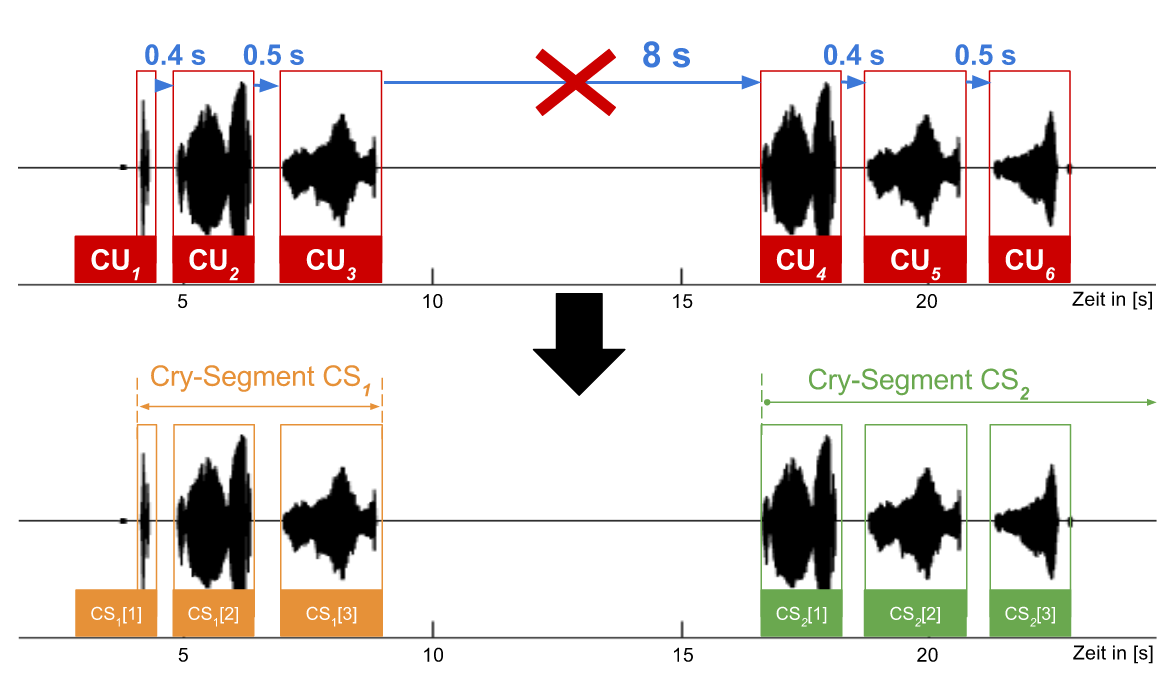
\includegraphics[width=1\textwidth]{bilder/segmentierung06.png}
	\caption{Ergebnis der Segmentierung mit einem Grenzwert von $t_s = \SI{6}{\second}$}
	\label{img:segmenting06}
\end{figure}

Das hier vorgestellte Vorgehen ist absichtlich möglichst einfach gehalten, damit der Sinn des Parameters $t_{s}$ leicht ersichtlich ist und somit von der medizinischen Fachkracht selbständig festgelegt werden kann. Schlussendlich ist eines der Hauptziele dieser Segmentierung, unnötige Berechnungen von Schmerz-Scores in den nachfolgenden Schritten zu vermeiden, so lange keine Cry-Units vorliegen. Das Ende eines Segmentes ist außerdem ein günstiger Zeitpunkt, um die Parameter des Kompressors im Pre-Processing auf Basis des RMS-Wertes des Segmentes zu aktualisieren (siehe Kapitel \ref{sec:preprocessing}). Trotz der Trivialität dieser laufenden Segmentierung liegt hier ein wichtiger Unterschied im Gegensatz zu vergleichbaren Systemen, wie zum Beispiel das von Cohen et al \cite{cohenCry}, bei dem die Entscheidung über Cry/not-Cry für Segmente mit einer festen Fenstergröße von 10 Sekunden vorgenommen wird. 

\section{Feature-Extraktion und Ableitung der Schmerzscore}
\label{sec:overviewPainRegression}

Das Erebnis der Segmentierung ist eine Litse an Cry-Segmenten $cs_0,  \ldots , c_n$. Diese Cry-Segmente bilden nun die Basis für die Ableitung der Pain-Score\footnote{Um Unklarheiten zu vermeiden, wird an dieser Stelle noch einmal darauf hingewiesen, dass mit \glqq Pain-Scale\grqq{} eine Scale, wie zum Beispiel die NIPS gemeint ist, und mit \glqq Pain-Score\glqq{} oder einfach nur \glqq Score\grqq{} die tatsächlich vergebene Punktzahl auf Basis der Bewertungskriterien der Pain-Scale}. Die medizinische Fachkraft, die das System verwendet, muss dabei zuerst die Wahl treffen, welche Pain-Scale verwendet werden soll. Das einfachste denkbare Vorgehen ist die Ableitung genau einer Pain-Score aus den globalen Eigenschaften eines Segmentes, wobei diese Ableitung erst vollzogen werden kann, sobald ein Segment abgeschlossen wurde und alle Informationen für dieses Segment vorliegen. Es wird also jedem Segment genau eine Pain-Score zugewiesen. Das Vorgehen wird am Beispiel der NIPS aus Tabelle \ref{tab:nips} verdeutlicht: Dabei steht die Abwesenheit von Weinen für null Punkte, \glqq mumbling\grqq{} (murmeln) für einen Punkt und \glqq vigorous\grqq{} (energisch) für zwei Punkte. Bei Abwesenheit von Lautäußerungen, also der Zeitraum zwischen den Segmenten, werden also keine Punkte = null Punkte vergeben. Ein Segment, dessen Qualität insgesamt als \glqq murmelnd\grqq{} bewertet wird, erhält einen Punkt, und ein Segment, welches als insgesamt als \glqq energisch\grqq{} bewertet wird, zwei Punkte. Das Problem ist offensichtlich: \glqq murmelnd\grqq{} und \glqq energisch\grqq{} sind subjektiv behaftete Begriffe und lassen sich nicht ohne weiteres aus den Eigenschaften eines Segmentes feststellen. 

Es werden zwei verschiedene Lösungs-Strategien für dieses Problem vorgestellt. 

\vspace{5mm}

\textbf{Strategie 1} \noindent\rule{0.83\linewidth}{0.3pt}\\
... löst das Problem mit Hilfe von \emph{Regression} (Siehe Kapitel \ref{sec:regression}):
\begin{enumerate}
 \item Man erstellt eine Datenbank mit Aufnahmen von kindlichen Lautäußerungen, die man  segmentiert.
 \item Man errechnet \glqq so viele \emph{objektiv} messabare Eigenschaften wie möglich\grqq{} für jedes Segment, wie zum Beispiel die insgesamte Länge, die durchschnittliche Länge der enthaltenen Cry-Units, durchschnittliche Tonhöhe usw.
 \item Man bittet medizinische Fachkräfte, für jedes Segment der Datenbank eine Score bezüglich einer Pain-Scale zu vergeben. Dadurch erhält man eine gelabelte Test-Datenbank.
 \item  Man verwendet einen \emph{Regressionsalgorithmus}, um den Zusammenhang zwischen den in Schritt 2 objektiv gemessenen Eigenschaften der Segmente und den in Schritt 3 vergebenen \emph{Scores} herzustellen. An dieser Stelle kann zum Beispiel die in Kapitel \ref{sec:multipleRegression} beschriebene multiple lineare Regression verwendet werden. Man erhält somit einen Regressor für jede Pain-Scale.
 \item Möchte man für neue, unbekannte Segmente die Pain-Score ableiten, nutzt man den entsprechenden Regressor.
\end{enumerate}
\noindent\rule{\linewidth}{0.3pt}

Das Vorteil dieses Vorgehens ist, dass das Problem der Übersetzung der objektiv messbaren Parameter in die subjektiv behafteten Begriffe überbrückt wird, indem die Regression direkt von den objektiv messbaren Parametern auf  die Pain-Score durchgeführt wird. Der Nachteil ist, dass eine Testdatenbank für jede Pain-Scale aufgebaut werden muss. Wird ein neue Pain-Scale eingeführt, muss der Regressor für diese Scale durch erneutes Labeln festgestellt werden. Ein weiterer Effekt der Abbildung des Problems als Regression ist, dass ein Regressor in einen kontinuierlichen Zahlenraum abbildet. Es sind also Regressionsergebnisse wie zum Beispiel $2.8$ denkbar. Diese \glqq bessere Auflösung\grqq{} kann als Vorteil betrachtet werden. Ist jedoch eine direkte Übersetzung der Pain-Scale inklusive der ganzzahligen Punktzahlen gewünscht, so stellt sich die Frage, ob eine $2.8$ auf- oder abzurunden ist.

\vspace{5mm}

\textbf{Strategie 2} \noindent\rule{0.83\linewidth}{0.3pt} \\
... löst das Problem mit Hilfe von Klassifizierung (Siehe Kapitel \ref{sec:classification}):
\begin{enumerate}
	\item und 2. entsprechen Strategie 1
	\stepcounter{enumi}
	\item Man sammelt alle subektiven Begriffe, die in Pain-Scales verwendet werden, wie zum Beispiel \glqq murmelnd\grqq , \glqq energisch\grqq , usw.
	\item Man bittet medizinische Fachkräfte, jedes Segment der Datenbann mit denjenigen Begriffen zu labeln, die die jeweilige Person für zutreffend hält. 
	\item  Man Verwendet einen \emph{Klassifizierungsgorithmus}, um einen Zusammenhang zwischen den in Schritt 2 festgestellten objektiv messbaren Eigenschaften der Segmente und den \emph{subjektiv behafteten Begriffen} zu finden. Man erhält somit einen Klassifikator für jedenBegriff, der binär in \emph{positive = zutreffend} und \emph{negative = nicht zutreffend} klassifiziert.
	\item Möchte man für neue, unbekannte Segmente die Pain-Score ableiten, so wird für jede Puntkzahl der Pain-Scale überprüft, ob für alle subjektiv beschreibenden Begriffe der entsprechende Klassifikator ein positive prognostiziert. Die Ableitung der Score ist somit ein weiters Klassifizierungsproblem, wobei eine Score einer Klasse entspricht und genau dann abgeleitet werden kann, wenn alle Vorraussetzungen für die Klasse erfüllt sind.
\end{enumerate}
\noindent\rule{\linewidth}{0.3pt}

Der Vorteil dieser Methode ist, dass auch zum Zeitpunkt der Erstellung der Testdatenbank unbekannte Pain-Scales zu einem späteren Zeitpunkt eingebunden werden können, insofern alle in dieser neuen Pain-Scale verwendeten subjektiv behafteten Begriffe bereits gelabelt vorliegen, weil sie auch in anderen Pain-Scales verwendet werden. Das Vorgehen erlaubt somit eine gewissen Flexibilität bezüglich zukünftig entwickelter Pain-Scales. Der Nachteil dieser Methode ist, dass durch die Umwandlung der eigentlich quantitativ geordenten Score einer Pain-Scale in qualitative Klassen aus einem implizit als Regression zu betrachtenden Problem ein Klassifizierungsproblem macht. Dies wirft neue Fragen auf, wie zum Beispiel: Angenommen, bei einer fiktiven Pain-Scale wird jede Score mit jeweils drei subjektiv behafteten Begriffen beschrieben, und bei der Klassifizierung eines Segmentes wird festgestellt, dass für jede Punktzahl genau zwei der drei Begriffe erfüllt werden. Welche Score wird dann abeleitet? Ein anderes Beispiel wird am Beispiel der der NIPS-Score aus Tabelle \ref{tab:nips} verdeutlicht: Angenommen, ein Cry-Segment enthält hörbar \glqq starkes\grqq{} Schreien, es kann jedoch weder \glqq mumbling (murmelnd) \grqq{} noch \glqq vigorous (energisch)\grqq{} abgeleitet werden. Demzufolgen müsste dieses Segment eine Score von 0 Punkten erhalten, wobei ein Mensch in dieser Situation eventuell \glqq stark\grqq{} zu \glqq heftig\grqq{} uminterpretieren und 2 Punkte vergeben würde.  Strategie 1 ist weniger anfällig für dieses Problem.

In jedem Fall werden medizinische Fachkräfte benötigt, um das Labeling der Cry-Segmente durchzuführen, was aus Zeitgründen im Rahmen dieser Arbeit nicht möglich ist. Die Aquise von Audioaufnahmen von Babys sowie das Labeling der Aufanhmen erfodern nicht nur Zeit, sondern das Fachwissen über das Führen und die Auswerten von Interviews.

\subsection{Extrahierung von Eigenschaften}
\label{sec:segmentFeatures}

Im vergangenen Kapitel wurde erläutert, dass die Basis für die Ableitung einer Pain-Score für ein Segment die Extraktion von \glqq so vielen Features wie möglich\grqq{} ist. In diesem Kapitel wird präzisiert, welche Features gemeint sind.  Varallyay \cite[S. 16 - 17]{cry_thesis} schlägt vor, drei Kategorien an Features zu betrachten: (1.) dem Zeitbereich, (2.) dem Frequenzbereich, und (3.) Melodie-bezogene Attribute. Diese Kategorisierung wird übernommen.

In Kapitel \ref{sec:acousticModel} wurde beschrieben, welche Features in der medizinischen Schreiforschung typischerweise extrahiert werden. In Kapitel \ref{sec:cryDiscussion} wurde diskutiert, dass (1.) nicht bewiesen ist, welche Features die \glqq wichtigsten\grqq{} sind und (2.) keine Einigung darüber herrscht, wie genau bestimmte Features zu berechnen sind. An dieser Stelle werden daher Berechnungsvorschriften für eine umfassende Auswahl an Features vorgestellt. Die Features basieren auf den Ideen, die in Kapitel \ref{sec:acousticModel} vorgestellt wurden, und erweitern diese logisch. Welche von diesen Features tatsächlich im Zusammenhang mit Schmerz stehen, lässt sich erst in der anschließenden Nutzung der Features zur Regression oder Klassifizierung der Pain-Scales feststellen, welche jedoch im Rahmen dieser Arbeit nicht durchgeführt werden kann.

%Viele der hier vorgestellten Features sind solche, die in der medizinischen Schreiforschung zur Analyse kindlicher Lautäußerungen genutzt wurden, jedoch in den meisten Fällen nicht computergestützt, sondern manuell ausgewertet wurden. Das hat zur Folge, dass die Features (1.) nicht mathematisch, sondern nur wörtlich beschrieben wurden, und (2.) einige Eigenschaften, die eigentlich trivial zu berechnen sind, ausgelassen wurden. Der vermutete Grund dafür ist, die Menge an Features überschaubarer zu halten. So wurden in einigen Veröffentlichungen beispielsweise häufig das Maximum, Minimum und Durchschnitt der Tonhöhen aller Cry-Units des Segmentes gemessen, in Bezug auf die Längen der Cry-Units jedoch nur der Durchschnitt (Beispiel: LaGasse et al \cite[S. 85]{parentalPerception}). Da in dieser Arbeit jedoch die Auslese der tatsächlich zu verwendenden Feautes zur Ableitung der Pain-Scores automatisiert durch einen Regressions oder Klassifizierungs-Algorithmus geschehen wird, gibt es keinen Grund, die Anzahl an Features von vorneherein zu begrenzen.  Auf Basis der eingeführten Datentypen Cry-Unit $CU$ aus Gleichung \ref{eq:cry-Unit} und Cry-Segment $[CS]$ \ref{eq:cry-segment} können die Features mathematisch definiert werden. Die nachfolgende Übersicht die nach Wissen des Autors der erste Versuch, eine umfassendere Menge von Features, die in der medizinischen Schreiforschung verwendet werden, mathematisch zu notieren.

\subsubsection{Features des Zeitbereiches}

Mit Features des Zeitbereiches sind solche gemeint, die sich allein aus Kenntnis der Cry-Units des Segments gewinnen lassen, wie beispielsweise die durchschnittliche Länge der Cry-Units, durchschnittliche Pause zwischen den Cry-Units, das relative Verhältnis von Cry-Units zu Pausen usw. Die folgenden Features werden konnkret definiert. In diesem Kapitel gilt die Konvention, dass eine Cry-Segment $cs$ insgesamt $N$ Cry-Units enthält, die Indexierung wird mit $0 \ldots N-1$ definiert.

\begin{description}
\item[Segment-Length: ] Zeitliche Länge des Segmentes:
\begin{equation}
\text{Segment-Length}(cs) = cs[N-1].end - cs[0].start
\label{eq:segment_length}
\end{equation}

\item[Density: ] Relativer Anteil der Cry-Units an der Länge des Segmentes (\glqq Dichte\grqq{})
\begin{equation}
\text{Density}(cs) = \frac{\sum_{i = 0}^{N-1} \lambda(cs[i])}{\text{Segment-Length}(cs)}
\end{equation}

\item[Tempo:] Das Verhältnis zwischen der Dauer des Segmentes und der Anzahl der Cry-Units. Dieses Feature wird von LaGasse et al \cite[S. 85]{parentalPerception} als \emph{Utterances} bezeichnet.

\begin{equation}
\text{Tempo}(cs) =  \frac{N}{\text{Segment-Length}(cs)}
\end{equation}

\item[Statistics of Cry-Units:] Statistische Auswertungen bezüglich der \emph{Länge der Cry-Units} $\text{stats}_{cu}(cs)$: Durchschnitt, Median, Minimum, Maximum und Standardabweichung der Cry-Units. Das $\text{mean}_{cu}(cs)$-Feature wird von LaGasse et al \cite[S. 85]{parentalPerception} und vielen weiteren Schreiforschern als \emph{Mean Duration} bezeichnet.

\begin{equation}
\text{stats}_{cu}(cs) = 
\begin{dcases}
\text{mean}_{cu}(cs) = \meani_{i = 0 \ldots N-1}\{\lambda(cs[i])\} \\
\text{median}_{cu}(cs) = \mediani_{i = 0 \ldots N-1}\{\lambda(cs[i])\} \\
\text{min}_{cu}(cs) = \mini_{i = 0 \ldots N-1}\{\lambda(cs[i])\} \\
\text{max}_{cu}(cs) = \maxi_{i = 0 \ldots N-1}\{\lambda(cs[i])\} \\
\sigma_{cu}(cs) =  \sigma_{i = 0 \ldots N-1}\{\lambda(cs[i])\} 
\end{dcases}
\label{eq:featuresOfCryUnits}
\end{equation}

\item[Statistics of Bursts:]\footnote{Erläuterung zum Begriff \emph{Burst} in  \ref{sec:acousticModel})} Die in Gleichung \ref{eq:featuresOfCryUnits} definierten Features können ebenso in Bezug auf die \emph{Längen der Bursts} errechnet werden, in dem in jeder Gleichung $\lambda(cs[i])$ ersetzt wird durch $cs[i].start - cs[i-1].start$. Die Indexierung muss auf $i = 1 ,\ldots, N-1$ begrenzt werden.

\begin{equation}
\text{stats}_{burst}(cs) = 
\begin{dcases}
\text{mean}_{burst}(cs) = \meani_{i = 1 \ldots N-1}\{cs[i].start - cs[i-1].start\} \\
\text{median}_{burst}(cs) = \mediani_{i = 1 \ldots N-1}\{cs[i].start - cs[i-1].start\} \\
\ldots
\end{dcases}
\label{eq:featuresOfBursts}
\end{equation}

\item[Statistics of Pauses:] Nach dem selben Muster werden die statistischen Auswertungen bezüglich der  \emph{Längen der Pausen} ermittelt. Eine Pause entspricht in diesem Zusammenhang der Distanz zweier aufeineraderfolgenden Cry-Units, welche in Kapitel \ref{sec:CryUnit} definiert wurde.

\begin{equation}
\text{stats}_{pause}(cs) = 
\begin{dcases}
\text{mean}_{pause}(cs) = \meani_{i = 1 \ldots N-1}\{d(cs[i-1],cs[i])\} \\
\text{median}_{pause}(cs)  = \ldots
\end{dcases}
\end{equation}

\item[Statistics of Energies:] Zunächst wird die Liste aller in den Cry-Units enthaltenen Signalfenster definiert nach Gleichung \ref{eq:windowsOfSegment}. Eine Cry-Unit hat die Signalfenster $cu.windows = x_0[\;],\ldots,x_m[\;]$

\begin{equation}
x_{seg}[\; ] = cs[0].windows[0] \;  , \; \ldots \; , \; cs[N-1].windows[m] 
\label{eq:windowsOfSegment}
\end{equation}

Die Liste $x_{seg}[\; ]$ hat $R$ Elemente, die Indexierung wird definiert mit $0, \ldots, R-1$. Gleichung \ref{eq:energyStats} definiert die Features bezüglich der MSV-Werte (\glqq Lautstärken\grqq ) des Segmentes. Der MSV-Wert als Maß des durchschnittlichen Energiegehaltes wurde in Gleichung \ref{eq:msv} definiert.

\begin{equation}
\text{stats}_{msv}(cs) = 
\begin{dcases}
\text{mean}_{E}(cs) = \meani_{i = 0 \ldots R-1}\{MSV(x_{seg}[i])\} \\
\text{median}_{E}(cs)  = \ldots
\end{dcases}
\label{eq:energyStats}
\end{equation}

\end{description}

Diese statistischen Auswertungen bezüglich der Länge der Cry-Units und Bursts wurden beispielsweise von Zeskind et al \cite{rythmic} vorgenommen, wenn auch nicht Computer-gestützt. Es ist zu bemerken, dass in der klassischen Schreiforschung zeitliche Features im geringeren Maße in Betracht gezogen wurden als Features des Frequenz-Bereiches. Die einzigen zeitliche Features, die zum Beispiel von Wasz-Hockert et al \cite{25years}, Fuller \cite{threeCryTypes} und LaGasse et al\cite{parentalPerception} in Betracht gezogen wurden, sind \emph{die durchschnittliche Länge der Cry-Units} (hier $\text{mean}_{cu}(cs)$) und die \emph{Latenz zwischen Reiz und erster Cry-Unit}, welche nur auf Basis des Audiosignals nicht feststellbar ist. Sie werden an dieser Stelle trotzdem berechnet, da nicht auszuschließen ist, dass sie zur Ableitung des Schmerzgrades eine Bedeutung erfüllen. Die anschließende Nutzung der Features zur Regression/Klassifizierung wird Auskunft darüber geben, welchen Beitrag diese Features zur Schmerzdiagnose leisten können.

\subsubsection*{Features des Frequenzbereiches und der Melodie}

Mit Features des Frequenz-Bereiches sind diejenigen Features gemeint, die sich aus der Short Time Fourier Transformation der Cry-Units gewinnen lassen. Um die Features durch mathematische Formeln definieren zu können, wird zuerst das \emph{Spectrum des Segmentes} $X_{seg}[\;]$ nach Formel \ref{eq:specOfSegment} als die Liste aller Frequenz-Bereiche der Signalfenster der Cry-Units des Segmentes definiert. Die Indexierung von $X_{seg}[\;]$ läuft, wie bei $x_{seg}[\;]$ von $0 , \ldots , R-1$. Nach dem selben Muster wird wird das \emph{Cepstrum des Segmentes} $c_{seg}[\;]$ definiert.

\begin{equation}
X_{seg}[\; ] := \mathop{\forall}_{x_i[\;] \; \in \; x_{seg}} :\ |DFT\{x_i[\;] \cdot w[\;]\}|
\label{eq:specOfSegment}
\end{equation}

Die folgenden Features des Frequenzbereiches lassen sich mit den in dieser Arbeit vorgestellten Methoden berechnen:

\begin{description}
\item[Tensness:] Das Feature, welches in Kapitel \ref{sec:acousticModel} als \glqq Ratio2\grqq{} beschrieben wurde. Es wurde von Fuller \cite{threeCryTypes} eingeführt und beschreibt die Spannung des Vokaltraktes als Verhältnis der Energien oberhalb von 2000 \SI{2000}{\hertz} zu unter \SI{2000}{\hertz} . Wie bei den statistischen Auswertungen der Features des Zeitbereiches kann für das gesamte Segment der Durchschnitt, Median, Maximum, Minimum und Standardabweichung berechnet werden.

\begin{equation}
\text{stats}(Tensness) = 
\begin{dcases}
\text{mean}_{Tens}(cs) = \meani_{i=0\ldots R-1} \Big\{ \frac{\sum_{k=0}^{\SI{2000}{\hertz}} X_{sec}[i][k]}{\sum_{j=\SI{2000}{\hertz}}^{f_{s}} X_{sec}[i][j]} \Big\} \\
\text{median}_{Tens}(cs) = \ldots
\end{dcases}
\end{equation}

\item[Clarity: ] Wie in Kapitel \ref{sec:cepstrum-feature} erläutert wurde, lässt eine stark ausgebildete Spitze im oberen Cepstrum-Bereich auf ein stimmhaftes Signal schließen. Ein hoher Anteil stärkerer Cepstrum-Peaks lässt also auf vermehrt phonierte Laute schließen, geringere Cepstrum-Peaks auf dysphoniertere Laute (Siehe Kapitel \ref{sec:acousticModel}). Dieses Feature trifft Aussagagen über den Anteil dysphonierter Laute, die Standardabweichung ähnelt dem in Kapitel \ref{sec:acousticModel} vorgestellten \emph{Cry-Mode Changes}-Feature.

\begin{equation}
\text{stats}_{clarity}(cs) = 
\begin{dcases}
\text{mean}_{Clarity}(cs) = \meani_{i=0\ldots R-1} \Big\{ Ceps_{mag}(c_{seg}[i])  \Big\} \\
\text{median}_{Clarity}(cs) = \ldots
\end{dcases}
\end{equation}
	
	
\end{description}

Alle weiteren Features, die in Kapitel \ref{sec:acousticModel} vorgestellt wurden und sich auf den Frequenzbereich beziehen, lassen sich nicht mehr mit den in dieser Arbeit vorgestellten Methoden extrahieren. Entweder beziehen sie sich auf die Lage der Formanten, oder basieren auf der Feststellung der Grundtonhöhe. In dieser Arbeit konnten aus Platzgründen jedoch keine Methoden zur Extraktion dieser Informationen mehr vorgestellt. Gleiches gilt für die Feststellung des Melodieverlaufs, welche ebenfalls auf der Feststellung der Grundtonhöhe basiert. Das Muster, nach dem diese Features berechnet werden können, sollte aus den bisher vorgestellten Features ersichtlich sein. So lassen sich beispielsweise die Features bezüglich der Grundtonhöhe nach Formel \ref{eq:pitchFeatures} ableiten. Dabei sei $f_0(X_i[\;])$ eine idealisierte Funktion, welche die Grundtonhöhe $f_0$ für das Frequenzfenster $X_i[\;]$ berechnet. Da für die Definition der weiteren Features idealisierte ebenfalls Funktionen angenommen werden müssten, wird die Festlegung weiterer Features an dieser Stelle nicht fortgeführt. 

\begin{equation}
\text{stats}_{pitch}(cs) = 
\begin{dcases}
\text{mean}_{Pitch}(cs) = \meani_{i=0\ldots R-1} \Big\{ f_0(X_{seg}[i]) \Big\} \\
\text{median}_{Pitch}(cs) = \ldots
\end{dcases}
\label{eq:pitchFeatures}
\end{equation}

\subsubsection*{Diskussion}

Bei allen vorgestellten Features handelt es sich, nach dem Vorbild der in Kapitel \ref{sec:acousticModel} vorgestellten Features der klassischen Schreiforschung, um solche, bei denen die Reihenfolge der Cry-Units nicht mit in Betracht gezogen wird. Angenommen, ein Segment besteht aus $n$ Cry-Units, wobei genau eine hälfte der  Cry-Units kurz und die andere hälfte der Cry-Units lang ist. Das $\text{stats}_{cu}(cs)$-Feature wird bezüglich des Durcschnittes, Minimum, Maximum etc. die selben Werte berechnen, unabhängig davon, ob sich die kurzen Cry-Units allesamt am Beginn des Segmentes, am Ende des Segmentes oder mit den langen Cry-Units durchmischt befinden. Bei der anschließenden Nutzung der Features zu Regression/Klassifizierung wird sich zeigen, wie sehr sich diese Features zur Ableitung von Pain-Scores eignen. Stellt sich heraus, dass sich die Features nicht eignen, ist es eventuell notwendig, die Position der Cry-Units in einer neuen Reihe von Features mit in Betracht zu ziehen.

\subsection{Ableitung der Pain-Score}
\label{sec:regressionPainScore}

Zu Beginn von Kapitel \ref{sec:overviewPainRegression} wurde gesagt, dass genau eine Score für ein Segment abgeleitet wird. Dies der einfachste denkbare Fall, welcher für einige Anwendungsfälle eventuell nicht ausreichend ist: 
\begin{enumerate}
\item Kann die Score erst nach der Beendigung eines Segmentes abgeleitet werden, was in einigen Kontexten möglicherweise zu spät ist. So kann es notwendig sein, bereits eine Score abzuleiten, bevor das Segment beendet wurde, um zum Beispiel das schnelle Reagieren auf akuten und starken Schmerz zu ermöglichen.
\item Falls der Schmerz innerhalb eines Segmentes stark ab- oder zunimmt, ist dieser Verlauf nicht erkennbar. Es würde lediglich der \glqq durchschnittliche Schmerz\grqq{} des Segmentes abgeleitet werden.
\end{enumerate}

Das vorgestellte Prinzip wird daher erweitert, indem ein Aktualisierungsintervall $t_{act}$ und Beobachtungszeitraume $t_{obs}$ eingeführt wird.

 Die Grundlegende Idee des Aktualsisierungsintervalles ist, bei einem momentan offenen Segment in regelmäßigen Abständen die Features abzufragen und direkt die Pain-Score abzuleiten, um Zwischenergebnisse zu erhalten. Der am häufigsten umsetzbare Fall ist, ein Aktualisierung nach jeder neu dem Segment hinzgefügten Cry-Unit vorzunehmen. Der am wenigsten häufige Fall ist der bereits genannte, die Aktualisierung erst bei Beendingung eines Segmentes durchzuführen. An den in Kapitel \ref{sec:segmentFeatures} vorgestellten Formeln ändert dies nichts, wenn zum Aktualisierungszeitpunkt das Ende des Segmentes angenommen wird. Wird die Entscheidung über die Aktualisierungshäufigkeit der medizinischen Fachkraft überlassen, empfiehlt es sich, den Parameter möglichst einfach verstehbar zu machen, in dem man einen festen Intervall $t_{act}$ festlegen lässt. Ein $t_{act}$ von beispielsweise \SI{10}{\second} bedeutet, dass alle 10 Sekunden ein neuer Pain-Score für ein Segment berechnet wird. Die Beendigung eines Segmentes würde in jedem Fall eine Ableitung der Pain-Score auslösen und einen \glqq erzwungenen Aktualisierungszeitpunkt\grqq{} darstellen. Es ist denkbar, das Aktualisierungsintervall fest an eine Pain-Scale zu binden. Die CRIES-Scale ist beispielsweise für das post-operative Monitoring gedacht und benötigt somit möglicherweise weniger häufige Aktualisierungen als der DAN, welcher zur Schmerzdiagnostik während einer Operation eingesetzt werden kann. \cite[S. 98]{painInNeonates}

Die Idee hinter der Festlegung des Beobachtungszeitraumes ist die Verkürzung des Zeitraumes, der zur Feature-Berechnung verwendet wird. Es gibt Eigenschaften, die sich implizit auf den gesamten Zeitraum \emph{Beginn des Segmentes} bis \emph{Aktualisierungs-Zeitpunkt} beziehen, wie beispielsweise die \emph{Zeitliche Länge des Segmentes} aus Formel \ref{eq:segment_length}. Dieser Zeitraum ist gleichzeitig der längst mögliche Zeitraum innerhalb eines Segmentes. Es ist jedoch auch möglich, kürzere Beobachtungszeiträume zu wählen. Dies hat zur Folge, dass die ersten Cry-Units des Segmentes ausgelassen werden, die außerhalb des Beobachtungszeitraumes liegen. Ist der Beobachtungszeitraum länger als die momentane Länge des Segmentes, werden die Berechnungen für das gesamte Segment durchgeführt. So können zeitliche Veränderungen der Pain-Score innerhalb eines Segmentes detaillierter dargestellt werden. Die in Kapitel \ref{sec:painScores} beschriebenen Pain-Scales geben wenig Informationen über \glqq typische Beobachtungszeiträume von Pain-Scales\grqq{}, da sie in den meisten Fällen in den Anleitungen nicht beschrieben werden. Bei der FLACC-Scale wird empfohlen, das Baby eine bis fünf Minuten zu beobachten.\cite{flacc} Es gibt keine belastbare Grundlagen, um Werte für $t_{obs}$ vorzuschalgen. Wie bei der Festlegung des Aktualisierungsintervalls ist es möglich, den Wert $t_{obs}$ von den medizinischen Fachkräften selbstständig festlegen zu lassen, oder fest an die verwendete Pain-Scale zu binden. Eine weitere Variante ist, $t_{obs}$ an den Wert des Parameters zu binden $t_{act}$, damit das medizinische Personal nur einen Wert festlegen muss. Ein Verhältnis von $t_{obs} = k \cdot t_{act}$ würde mit $k=1$ nicht-überlappende Beobachtungszeiträume und  mit $k=2$ überlappende Beobachtungszeiträume erzeugen.

\section{Visualisierung}
\label{sec:visualisation}